\documentclass[11pt]{article}
\usepackage{amsmath,amssymb,array,booktabs,longtable,geometry,fontspec,xcolor}
\usepackage{tikz}\usetikzlibrary{arrows.meta}
\usepackage[hidelinks]{hyperref}
\definecolor{claimlink}{RGB}{25,70,150}
\newcommand{\pvar}[2]{\hyperlink{#1-P#2}{\textcolor{claimlink}{P_{#2}}}}
\newcommand{\pvartarget}[2]{\raisebox{\ht\strutbox}{\hypertarget{#1-P#2}{}}}
\makeatletter
\newenvironment{derivation}
  {\begin{list}{}{\setlength{\leftmargin}{2.6em}\setlength{\labelwidth}{2.2em}%
    \setlength{\labelsep}{0.4em}\setlength{\itemsep}{2pt}\setlength{\parsep}{0pt}%
    \setlength{\topsep}{6pt}\@beginparpenalty\@M\@itempenalty\@M%
    \interlinepenalty\@M\raggedright}}
  {\end{list}}
\newcommand{\breakrow}[1]{\@itempenalty\z@\item[#1]\@itempenalty\@M}
\newcommand{\keepwithnext}{\@endparpenalty\@M}
\makeatother
\clubpenalty=10000
\widowpenalty=10000
\newcommand{\gloss}[1]{\enspace---\enspace{\small\itshape #1}}
\geometry{margin=1in}
\setlength{\emergencystretch}{3em}
\frenchspacing
\setmainfont{FreeSerif}[Extension=.otf,UprightFont=*,BoldFont=*Bold,
  ItalicFont=*Italic,BoldItalicFont=*BoldItalic,Ligatures=TeX]
\setmonofont{DejaVuSansMono}[Extension=.ttf,UprightFont=*,BoldFont=*-Bold,
  ItalicFont=*-Oblique,BoldItalicFont=*-BoldOblique,Scale=MatchLowercase]
\newfontfamily\hebrewfont{FreeSerif}[Extension=.otf,UprightFont=*,BoldFont=*Bold,
  ItalicFont=*,BoldItalicFont=*Bold,Script=Hebrew]
\newfontfamily\syriacfont{FreeSans}[Extension=.otf,UprightFont=*,BoldFont=*Bold,
  ItalicFont=*,BoldItalicFont=*Bold,Script=Syriac]
\newfontfamily\symbolfont{FreeSerif}[Extension=.otf,UprightFont=*,BoldFont=*Bold,
  ItalicFont=*,BoldItalicFont=*Bold]
\XeTeXinterchartokenstate=1
\newcommand{\fontrange}[3]{\count255=#2\relax
  \loop\XeTeXcharclass\count255=#1\relax\ifnum\count255<#3\relax
  \advance\count255 by 1\repeat}
\newXeTeXintercharclass\hebrewclass
\fontrange\hebrewclass{"0590}{"05FF}
\newXeTeXintercharclass\syriacclass
\fontrange\syriacclass{"0700}{"074F}
\newXeTeXintercharclass\symbolclass
\fontrange\symbolclass{"1D2C}{"1D6A}
\fontrange\symbolclass{"22C0}{"22C3}
\XeTeXinterchartoks 0 \hebrewclass {\begingroup\hebrewfont}
\XeTeXinterchartoks 4095 \hebrewclass {\begingroup\hebrewfont}
\XeTeXinterchartoks \hebrewclass 0 {\endgroup}
\XeTeXinterchartoks \hebrewclass 4095 {\endgroup}
\XeTeXinterchartoks \hebrewclass \syriacclass {\endgroup\begingroup\syriacfont}
\XeTeXinterchartoks \hebrewclass \symbolclass {\endgroup\begingroup\symbolfont}
\XeTeXinterchartoks 0 \syriacclass {\begingroup\syriacfont}
\XeTeXinterchartoks 4095 \syriacclass {\begingroup\syriacfont}
\XeTeXinterchartoks \syriacclass 0 {\endgroup}
\XeTeXinterchartoks \syriacclass 4095 {\endgroup}
\XeTeXinterchartoks \syriacclass \hebrewclass {\endgroup\begingroup\hebrewfont}
\XeTeXinterchartoks \syriacclass \symbolclass {\endgroup\begingroup\symbolfont}
\XeTeXinterchartoks 0 \symbolclass {\begingroup\symbolfont}
\XeTeXinterchartoks 4095 \symbolclass {\begingroup\symbolfont}
\XeTeXinterchartoks \symbolclass 0 {\endgroup}
\XeTeXinterchartoks \symbolclass 4095 {\endgroup}
\XeTeXinterchartoks \symbolclass \hebrewclass {\endgroup\begingroup\hebrewfont}
\XeTeXinterchartoks \symbolclass \syriacclass {\endgroup\begingroup\syriacfont}
\usepackage{newunicodechar}
\newunicodechar{🡒}{→}
\title{Spirit baptism — at conversion, after it, or in the sacraments}
\author{\credit{TestimonyArguments.SpiritBaptism}}
\date{Generated by \texttt{lake exe argtex}}
\newcommand{\credit}[1]{\ifcsname credit@#1\endcsname\csname credit@#1\endcsname\fi}
\newcommand{\creditline}[1]{\ifcsname credit@#1\endcsname{\centering\credit{#1}\par\medskip}\fi}
\InputIfFileExists{credits.def}{}{}
\begin{document}
\maketitle
\noindent This is one argument of the Testimony library, printed on its own. The library prints every argument together in \texttt{arguments.pdf}. This one is set as its Lean source sets it: the module docstrings as prose, in the order they are written, and under each one the package, line of reason, countermodel or result it introduces. Atoms are numbered propositional variables, numbered once per argument, so a variable means the same claim in every position within it; the legend gives each one's claim, its classification, the tradition that holds it and the source that carries it.

\noindent Nothing here asserts that the premises are true --- only that the conclusion does or does not follow from them.

\tableofcontents
\clearpage
\section*{Spirit baptism — at conversion, after it, or in the sacraments}
\addcontentsline{toc}{section}{Spirit baptism — at conversion, after it, or in the sacraments}

\subsection*{Spirit baptism: the question and its answers}
\addcontentsline{toc}{subsection}{Spirit baptism: the question and its answers}
John the Baptist told the crowds at the Jordan that one was coming after him who was greater than he:

\begin{quote}
“I have baptized you with water, but he will baptize you with the Holy Spirit.” (Mark 1:8)

\end{quote}
Every Christian tradition agrees that Jesus is the one John meant. They do not agree on when he does it. Is the baptism with the Spirit something every Christian receives in becoming a Christian? Or is it a second experience, to be sought after conversion? Or is the Spirit given in the sacraments, in water baptism and in confirmation? This argument sets out the answers, each in the words of those who give it, and checks what follows from each.

The question is asked mostly \emph{among} Protestants, and it concerns what follows conversion, not justification itself. So it is an argument of its own, and not a party to the sola fide dispute. Its sides do not line up with that dispute’s either. Lutherans and Rome have confessed together “that sinners are justified by faith in the saving action of God in Christ” (the \emph{Joint Declaration}, §25), and that the Lutheran teaching it states “does not fall under the condemnations from the Council of Trent” (§41). Baptists, Pentecostals and the holiness churches did not sign it. Lutherans, the Reformed, Baptists, Pentecostals and the holiness churches all hold that faith \emph{alone} justifies. Rome does not teach that, but agreed in the \emph{Joint Declaration} that the Lutheran teaching is not condemned by Trent. On Spirit baptism the lines fall elsewhere. Lutherans stand partly with Rome, because they hold that the Spirit is given in water baptism, and Baptists stand with the Reformed.

\subsubsection*{Three answers, four positions}
Paul wrote to the church at Corinth, “in one Spirit we were all baptized into one body” (1 Corinthians 12:13). James Dunn, in \emph{Baptism in the Holy Spirit}, and John Stott read that verse as the baptism in the Spirit that Christ gives. It is part of becoming a Christian, they hold, so there is no second one to seek.

Two traditions answer that there is a second, after conversion. This page calls them together \emph{the subsequence views}.

\begin{itemize}
  \item \textbf{The Pentecostal view.} The Assemblies of God, in a position paper of 2010, hold that at conversion the Spirit baptizes the believer into the body of Christ. On their reading 1 Corinthians 12:13 is baptism \emph{by} the Spirit: “the Holy Spirit is the instrument”. Then, in “a subsequent and distinct experience, Christ will baptize in the Holy Spirit”, as in Samaria (Acts 8) and at Ephesus (Acts 19), to empower the believer. Robert Menzies and Roger Stronstad reach the second gift from Luke rather than from Paul: Luke’s baptism in the Spirit, they hold, is prophetic empowerment.
  \item \textbf{The holiness view.} \emph{Entire sanctification} is a second work of grace after conversion, in which the believer is cleansed from sin and made perfect in love. The holiness view holds that this is the baptism with the Spirit. The Church of the Nazarene confesses that entire sanctification “is wrought by the baptism with or infilling of the Holy Spirit” (\emph{Manual} 2023, Article X). The view is contested from within its own tradition. John Wesley, whose teaching on the second work the holiness churches carry on, held the second work and declined the name: “they all ‘received the Holy Ghost’ when they were justified”. In 2010 the faculty of the Nazarene seminary, who keep entire sanctification, wrote that they no longer hold that reading of the Spirit’s baptism to be exegetically tenable.
\end{itemize}
The third answer is Rome’s. The Spirit is given in water baptism, “new birth in the Holy Spirit”, and in confirmation, “the full outpouring of the Holy Spirit as once granted to the apostles on the day of Pentecost”. Lutherans hold the first half, and keep confirmation as a rite, not a sacrament. This is a later gift too, but a sacramental one, not a second baptism beyond the sacraments. The Catholic charismatic renewal speaks of a “baptism in the Spirit” of its own, and it is not encoded here.

Two questions are not encoded yet.

\begin{itemize}
  \item \textbf{Tongues.} The Assemblies of God hold that speaking in tongues is the \emph{initial evidence} of Spirit baptism, the first outward sign that a believer has received it (their paper, summary statement 5). To rate that claim honestly needs a reader who grants the subsequence view and still denies the evidence doctrine, since everyone who denies subsequence denies it trivially. Pentecostal dissenters are known, Gordon Fee and F. F. Bosworth among them, but their words could not be verified. So the claim is left out rather than rated from memory.
  \item \textbf{Paul’s word and Luke’s.} “Baptized in the Spirit” may not mean the same in 1 Corinthians 12:13 as in Acts. Menzies grants that Paul’s baptism in the Spirit comes at conversion, and holds that Luke’s is a different, later gift. If he is right, the conversion view and the Pentecostal view are partly answering different questions. The encoding uses one word for both, and a dilemma over the word is the natural next step.
\end{itemize}
\subsubsection*{Where it turns}
The argument turns on the Acts narratives. The Pentecostal view holds that they are a pattern for believers today. Stott reads them as unrepeatable transitions, which set no pattern. When the four views are weighed against one another, no view wins outright. Each is answered by a rival it answers in turn, and every view rests somewhere on a claim rated \texttt{disputed}, the lowest rating, so the ratings cannot break the tie (\texttt{spirit\_\allowbreak{}baptism\_\allowbreak{}forces\_\allowbreak{}nothing}). That is not the same as any view being false. The views fall into two groups that can each be held together: the conversion and sacramental views, and the two subsequence views. Each view can be defended from inside its group, and no position holds views from both.

\subsubsection*{The questions the later chapters take}
\begin{itemize}
  \item \textbf{What does each view rest on, and can Acts be read as Stott reads it?} Each view is set out from its own texts and checked. The Pentecostal view cannot read Acts as transitions at all, and the variety of Acts meets its pattern at a step the Assemblies of God contest (“Each view from its own texts, and what Acts can carry”).
  \item \textbf{Weighed against each other, which view wins?} None wins outright. Four pairs of views answer each other, and every view can be defended (“Weighing the four views”).
  \item \textbf{What does each claim mean, and who holds it?} Every claim, with its source and its rating (“Appendix: the claims and their sources”).
\end{itemize}
\subsection*{Each view from its own texts, and what Acts can carry}
\addcontentsline{toc}{subsection}{Each view from its own texts, and what Acts can carry}
Each of the four views starts from a text and a reading of it. Dunn and Stott start from Paul: “in one Spirit we were all baptized into one body” (1 Corinthians 12:13), read as the baptism Christ gives every believer. From that, Spirit baptism comes at conversion, and if it comes at conversion there is no second one to seek. The Assemblies of God start from the same verse read another way, as the Spirit baptizing the believer into the body, and then from Luke: in Samaria and at Ephesus people who had believed and been baptized received the Spirit afterwards, when the apostles laid hands on them (Acts 8:14–17; 19:1–7). Read as a pattern of empowerment for believers today, those episodes give a second baptism in the Spirit to seek. The Church of the Nazarene starts from entire sanctification, the second work of grace, and holds that it is wrought by the baptism with the Spirit. Rome starts from Peter at Pentecost:

\begin{quote}
“Repent and be baptized every one of you in the name of Jesus Christ for the forgiveness of your sins, and you will receive the gift of the Holy Spirit.” (Acts 2:38)

\end{quote}
The Spirit is given in water baptism and fully in confirmation, so there is no second baptism to seek beyond the sacraments.

Each view, granted its premises, delivers its conclusion, and each can be held without contradiction (\texttt{conversion\allowbreak{}Case\_\allowbreak{}establishes}, \texttt{pentecostal\allowbreak{}Case\_\allowbreak{}establishes}, \texttt{holiness\allowbreak{}Case\_\allowbreak{}establishes}, \texttt{sacramental\allowbreak{}Case\_\allowbreak{}establishes}). That much is a check of validity. It does not show that any of the readings is right, and every reading of 1 Corinthians 12:13 here is rated \texttt{disputed}, because each side rejects the other’s.

\subsubsection*{What Acts can carry}
So much rests on how Luke’s narratives are read that two further arguments are set out about them. The first is from the variety of Acts. The Spirit falls on Cornelius’s household as they hear the word, before they are baptized (10:44); at Pentecost it is promised with baptism (2:38); in Samaria and at Ephesus it comes later, with hands laid on (8:17; 19:6). Acts gives no one order, so no one episode is the pattern (\texttt{variety\allowbreak{}Case\_\allowbreak{}establishes}). The second is Stott’s. The later reception of the Spirit in Samaria and at Ephesus marks steps in the gospel’s spread, unrepeatable transitions, and so sets no norm for believers today (\texttt{transition\allowbreak{}Case\_\allowbreak{}establishes}).

A Pentecostal cannot also read Acts as Stott does. The view’s own premise is that the narratives are a pattern, and Stott’s reading denies it, so the two claims, taken at their word, cannot both be held (\texttt{pentecostal\_\allowbreak{}cannot\_\allowbreak{}read\_\allowbreak{}acts\_\allowbreak{}as\_\allowbreak{}transitions}). Read as a pattern, the narratives then collide with the variety of Acts, at one step: from Acts 10 and 2:38 to “no one episode is the pattern”. The Assemblies of God deny that step. They grant Acts 10, and their paper lists Acts 10:44–46 as evidence \emph{for} a later experience (\texttt{where\allowbreak{}The\allowbreak{}Variety\allowbreak{}Meets\allowbreak{}The\allowbreak{}Pattern}). So the Pentecostal view must read Acts as a pattern and answer its variety, and its answer is a reading of Acts 10 that the step’s rating records as disputed.

The other views’ readings of Acts are not checked here: Stott’s reason for holding that Luke’s narratives set no order for later believers, Dunn’s argument that the Samaritans were not yet believers before they received the Spirit, and Rome’s reading of Acts 8:17 and 19:6 as confirmation (Catechism 1288). The chapter “Weighing the four views” sets the four views against one another.

\subsubsection*{How this is checked}
\paragraph*{The conversion view}
\leavevmode\par\nobreak
\par\medskip\noindent\textbf{\texttt{corinthians\allowbreak{}To\allowbreak{}Conversion}}\par\nobreak\noindent
From 1 Corinthians 12:13, read as Christ baptizing in the Spirit, to Spirit baptism at conversion. Rated \texttt{disputed}, conservatively: the Assemblies of God deny its conclusion by denying a ground, the conversion reading.

\par\smallskip\noindent If each of these holds,
\begin{derivation}
  \item[(1)] \(\pvar{TestimonyArguments.SpiritBaptism}{1}\)\enspace 1 Corinthians 12:13 — in one Spirit we were all baptized into one body\gloss{consensus: 1 Cor 12:13}
  \item[(2)] \(\pvar{TestimonyArguments.SpiritBaptism}{5}\)\enspace 1 Corinthians 12:13 is the baptism in the Spirit Christ gives, received by every believer at conversion\gloss{disputed: \cite{dunn-baptism-holy-spirit-1970}; \cite{stott-baptism-fullness-1975}}
  \item[\(\therefore\)] \(\pvar{TestimonyArguments.SpiritBaptism}{13}\)\enspace Every believer is baptized in the Spirit at conversion
\end{derivation}
\noindent In symbols, the step is \((\pvar{TestimonyArguments.SpiritBaptism}{1} \land \pvar{TestimonyArguments.SpiritBaptism}{5}) \rightarrow \pvar{TestimonyArguments.SpiritBaptism}{13}\).
\par\medskip\noindent\textbf{\texttt{conversion\allowbreak{}Excludes\allowbreak{}ASecond}}\par\nobreak\noindent
If every believer is baptized in the Spirit at conversion, there is no second Spirit baptism to seek. Rated \texttt{disputed}: Menzies grants that Paul’s baptism in the Spirit comes at conversion and holds that Luke’s is a second gift, to be sought. Whether he denies this step or uses the word in two senses is not yet encoded.

\par\smallskip\noindent If each of these holds,
\begin{derivation}
  \item[(1)] \(\pvar{TestimonyArguments.SpiritBaptism}{13}\)\enspace Every believer is baptized in the Spirit at conversion\gloss{disputed: \cite{dunn-baptism-holy-spirit-1970}; \cite{stott-baptism-fullness-1975}}
  \item[\(\therefore\)] \(\lnot \pvar{TestimonyArguments.SpiritBaptism}{14}\)\enspace \emph{denied:} A baptism in the Spirit distinct from and after conversion is to be sought
\end{derivation}
\noindent In symbols, the step is \(\pvar{TestimonyArguments.SpiritBaptism}{13} \rightarrow \lnot \pvar{TestimonyArguments.SpiritBaptism}{14}\).
\par\medskip\noindent\textbf{\texttt{conversion\allowbreak{}Case}} --- At conversion (Dunn, Stott)\par\nobreak\noindent
\textbf{The conversion view}, as Dunn and Stott hold it: every believer is baptized in the Spirit at conversion, so there is no second Spirit baptism to seek.

\begin{derivation}
  \item[(1)] \(\pvar{TestimonyArguments.SpiritBaptism}{1}\)\gloss{1 Corinthians 12:13 — in one Spirit we were all baptized into one body}
  \item[(2)] \(\pvar{TestimonyArguments.SpiritBaptism}{5}\)\gloss{1 Corinthians 12:13 is the baptism in the Spirit Christ gives, received by every believer at conversion}
  \item[(3)] \((\pvar{TestimonyArguments.SpiritBaptism}{1} \land \pvar{TestimonyArguments.SpiritBaptism}{5}) \rightarrow \pvar{TestimonyArguments.SpiritBaptism}{13}\)
  \item[(4)] \(\pvar{TestimonyArguments.SpiritBaptism}{13} \rightarrow \lnot \pvar{TestimonyArguments.SpiritBaptism}{14}\)\gloss{\emph{would deny:} A baptism in the Spirit distinct from and after conversion is to be sought}
  \item[\(\vdash\)] \(\pvar{TestimonyArguments.SpiritBaptism}{13}\)\gloss{\emph{at issue:} Every believer is baptized in the Spirit at conversion}
  \keepwithnext
\end{derivation}
\emph{Grounded in scripture alone:} 1 Corinthians 12:13 — in one Spirit we were all baptized into one body.
\paragraph*{The Pentecostal view}
\leavevmode\par\nobreak
\par\medskip\noindent\textbf{\texttt{instrumental\allowbreak{}Reading\allowbreak{}Excludes\allowbreak{}Conversion}}\par\nobreak\noindent
The Pentecostal reading of 1 Corinthians 12:13 excludes the conversion reading: if the Spirit is the instrument baptizing into the body, the verse is not Christ baptizing in the Spirit. Rated \texttt{disputed}, conservatively: Dunn and Stott deny its conclusion by denying a ground, the instrumental reading.

\par\smallskip\noindent If each of these holds,
\begin{derivation}
  \item[(1)] \(\pvar{TestimonyArguments.SpiritBaptism}{1}\)\enspace 1 Corinthians 12:13 — in one Spirit we were all baptized into one body\gloss{consensus: 1 Cor 12:13}
  \item[(2)] \(\pvar{TestimonyArguments.SpiritBaptism}{6}\)\enspace 1 Corinthians 12:13 is baptism by the Spirit into the body, not Christ baptizing in the Spirit\gloss{disputed: \cite{assemblies-of-god-baptism-holy-spirit-2010}}
  \item[\(\therefore\)] \(\lnot \pvar{TestimonyArguments.SpiritBaptism}{5}\)\enspace \emph{denied:} 1 Corinthians 12:13 is the baptism in the Spirit Christ gives, received by every believer at conversion
\end{derivation}
\noindent In symbols, the step is \((\pvar{TestimonyArguments.SpiritBaptism}{1} \land \pvar{TestimonyArguments.SpiritBaptism}{6}) \rightarrow \lnot \pvar{TestimonyArguments.SpiritBaptism}{5}\).
\par\medskip\noindent\textbf{\texttt{acts\allowbreak{}To\allowbreak{}Second}}\par\nobreak\noindent
From the Acts narratives, read as a pattern of empowerment, to a second Spirit baptism to be sought. Rated \texttt{well\allowbreak{}Supported}: its rejecters deny a ground, not the step.

\par\smallskip\noindent If each of these holds,
\begin{derivation}
  \item[(1)] \(\pvar{TestimonyArguments.SpiritBaptism}{2}\)\enspace Acts 8:14–17 and 19:1–7 — believers, already baptized, receive the Spirit afterwards (so the Assemblies of God; Dunn denies they were yet believers)\gloss{disputed: \cite{assemblies-of-god-baptism-holy-spirit-2010}; Acts 8:14-17; Acts 19:1-7}
  \item[(2)] \(\pvar{TestimonyArguments.SpiritBaptism}{7}\)\enspace In Luke-Acts, baptism in the Spirit is prophetic empowerment, distinct from the gift Paul ties to conversion\gloss{disputed: \cite{menzies-lukes-understanding-2017}; \cite{menzies-empowered-witness-1994}; \cite{stronstad-charismatic-theology-1984}}
  \item[(3)] \(\pvar{TestimonyArguments.SpiritBaptism}{8}\)\enspace Luke’s narratives of receiving the Spirit are a pattern for believers today\gloss{disputed: \cite{stronstad-charismatic-theology-1984}; \cite{assemblies-of-god-baptism-holy-spirit-2010}}
  \item[\(\therefore\)] \(\pvar{TestimonyArguments.SpiritBaptism}{14}\)\enspace A baptism in the Spirit distinct from and after conversion is to be sought
\end{derivation}
\noindent In symbols, the step is \((\pvar{TestimonyArguments.SpiritBaptism}{2} \land \pvar{TestimonyArguments.SpiritBaptism}{7} \land \pvar{TestimonyArguments.SpiritBaptism}{8}) \rightarrow \pvar{TestimonyArguments.SpiritBaptism}{14}\).
\par\medskip\noindent\textbf{\texttt{pentecostal\allowbreak{}Case}} --- After conversion (Assemblies of God; Menzies, Stronstad)\par\nobreak\noindent
\textbf{The Pentecostal view}, as the Assemblies of God hold it: at conversion the Spirit baptizes into the body of Christ (1 Corinthians 12:13); in a subsequent and distinct experience Christ baptizes in the Spirit, as in Samaria and at Ephesus, for empowerment.

\begin{derivation}
  \item[(1)] \(\pvar{TestimonyArguments.SpiritBaptism}{1}\)\gloss{1 Corinthians 12:13 — in one Spirit we were all baptized into one body}
  \item[(2)] \(\pvar{TestimonyArguments.SpiritBaptism}{6}\)\gloss{1 Corinthians 12:13 is baptism by the Spirit into the body, not Christ baptizing in the Spirit}
  \item[(3)] \(\pvar{TestimonyArguments.SpiritBaptism}{2}\)\gloss{Acts 8:14–17 and 19:1–7 — believers, already baptized, receive the Spirit afterwards (so the Assemblies of God; Dunn denies they were yet believers)}
  \breakrow{(4)} \(\pvar{TestimonyArguments.SpiritBaptism}{7}\)\gloss{In Luke-Acts, baptism in the Spirit is prophetic empowerment, distinct from the gift Paul ties to conversion}
  \breakrow{(5)} \(\pvar{TestimonyArguments.SpiritBaptism}{8}\)\gloss{Luke’s narratives of receiving the Spirit are a pattern for believers today}
  \breakrow{(6)} \((\pvar{TestimonyArguments.SpiritBaptism}{1} \land \pvar{TestimonyArguments.SpiritBaptism}{6}) \rightarrow \lnot \pvar{TestimonyArguments.SpiritBaptism}{5}\)\gloss{\emph{would deny:} 1 Corinthians 12:13 is the baptism in the Spirit Christ gives, received by every believer at conversion}
  \item[(7)] \((\pvar{TestimonyArguments.SpiritBaptism}{2} \land \pvar{TestimonyArguments.SpiritBaptism}{7} \land \pvar{TestimonyArguments.SpiritBaptism}{8}) \rightarrow \pvar{TestimonyArguments.SpiritBaptism}{14}\)
  \item[\(\vdash\)] \(\pvar{TestimonyArguments.SpiritBaptism}{14}\)\gloss{\emph{at issue:} A baptism in the Spirit distinct from and after conversion is to be sought}
  \keepwithnext
\end{derivation}
\emph{Grounded in scripture alone:} 1 Corinthians 12:13 — in one Spirit we were all baptized into one body.
\par\medskip\noindent\textbf{\texttt{second\allowbreak{}Work\allowbreak{}Is\allowbreak{}The\allowbreak{}Baptism}}\par\nobreak\noindent
The holiness step: the second work of grace is the baptism with the Spirit, to be sought after conversion. Rated \texttt{disputed}: Wesley grants the second work and denies that it is “receiving the Holy Ghost”.

\par\smallskip\noindent If each of these holds,
\begin{derivation}
  \item[(1)] \(\pvar{TestimonyArguments.SpiritBaptism}{10}\)\enspace Entire sanctification is a second work of grace after justification\gloss{disputed: \cite[Articles of Faith, X, ¶10]{church-of-the-nazarene-manual-2023}; \cite[to Joseph Benson, 28 December 1770]{wesley-letters-1931}; \cite{bassett-white-paper-article-x-2010}}
  \item[\(\therefore\)] \(\pvar{TestimonyArguments.SpiritBaptism}{14}\)\enspace A baptism in the Spirit distinct from and after conversion is to be sought
\end{derivation}
\noindent In symbols, the step is \(\pvar{TestimonyArguments.SpiritBaptism}{10} \rightarrow \pvar{TestimonyArguments.SpiritBaptism}{14}\).
\par\medskip\noindent\textbf{\texttt{holiness\allowbreak{}Case}} --- A second work of grace (the holiness tradition)\par\nobreak\noindent
\textbf{The holiness view}, as the Church of the Nazarene confesses it: entire sanctification is a second work of grace, and it “is wrought by the baptism with or infilling of the Holy Spirit” (\emph{Manual} 2023, Article X). Contested from within its own tradition, by Wesley and by the Nazarene seminary faculty.

\begin{derivation}
  \item[(1)] \(\pvar{TestimonyArguments.SpiritBaptism}{10}\)\gloss{Entire sanctification is a second work of grace after justification}
  \item[(2)] \(\pvar{TestimonyArguments.SpiritBaptism}{10} \rightarrow \pvar{TestimonyArguments.SpiritBaptism}{14}\)
  \item[\(\vdash\)] \(\pvar{TestimonyArguments.SpiritBaptism}{14}\)\gloss{\emph{at issue:} A baptism in the Spirit distinct from and after conversion is to be sought}
  \keepwithnext
\end{derivation}
\emph{No premise here rests on scripture alone.}
\paragraph*{The sacramental view}
\leavevmode\par\nobreak
\par\medskip\noindent\textbf{\texttt{acts\allowbreak{}Two\allowbreak{}To\allowbreak{}The\allowbreak{}Sacraments}}\par\nobreak\noindent
From Acts 2:38, with the Spirit given in water baptism and fully in confirmation, to the Spirit given in the sacraments, not in an experience to be sought. Rated \texttt{disputed}, conservatively: Westminster, which holds that the grace of baptism is not tied to the moment of the rite, denies a ground, not the step.

\par\smallskip\noindent If each of these holds,
\begin{derivation}
  \item[(1)] \(\pvar{TestimonyArguments.SpiritBaptism}{4}\)\enspace Acts 2:38 — repent and be baptized, and you will receive the gift of the Spirit\gloss{consensus: Acts 2:38}
  \item[(2)] \(\pvar{TestimonyArguments.SpiritBaptism}{11}\)\enspace The Spirit is given in water baptism: new birth in the Holy Spirit\gloss{disputed: \cite[1262]{catholic-church-catechism-2000}; \cite[1265]{catholic-church-catechism-2000}; \cite[Small Catechism, Baptism, third part]{kolb-wengert-book-of-concord-2000}}
  \item[(3)] \(\pvar{TestimonyArguments.SpiritBaptism}{12}\)\enspace Confirmation gives the full outpouring of the Spirit, as at Pentecost and in Samaria\gloss{disputed: \cite[1302]{catholic-church-catechism-2000}; \cite[1288]{catholic-church-catechism-2000}}
  \item[\(\therefore\)] \(\pvar{TestimonyArguments.SpiritBaptism}{15}\)\enspace The Spirit is given in baptism and confirmation, not in a second baptism beyond the sacraments
\end{derivation}
\noindent In symbols, the step is \((\pvar{TestimonyArguments.SpiritBaptism}{4} \land \pvar{TestimonyArguments.SpiritBaptism}{11} \land \pvar{TestimonyArguments.SpiritBaptism}{12}) \rightarrow \pvar{TestimonyArguments.SpiritBaptism}{15}\).
\par\medskip\noindent\textbf{\texttt{sacraments\allowbreak{}Exclude\allowbreak{}ASeeking}}\par\nobreak\noindent
If the Spirit is given in the sacraments, there is no second Spirit baptism to seek beyond them. Rated \texttt{disputed}, conservatively: the Catholic charismatic renewal is its natural contester, not yet cited.

\par\smallskip\noindent If each of these holds,
\begin{derivation}
  \item[(1)] \(\pvar{TestimonyArguments.SpiritBaptism}{15}\)\enspace The Spirit is given in baptism and confirmation, not in a second baptism beyond the sacraments\gloss{disputed: \cite[1302]{catholic-church-catechism-2000}}
  \item[\(\therefore\)] \(\lnot \pvar{TestimonyArguments.SpiritBaptism}{14}\)\enspace \emph{denied:} A baptism in the Spirit distinct from and after conversion is to be sought
\end{derivation}
\noindent In symbols, the step is \(\pvar{TestimonyArguments.SpiritBaptism}{15} \rightarrow \lnot \pvar{TestimonyArguments.SpiritBaptism}{14}\).
\par\medskip\noindent\textbf{\texttt{sacramental\allowbreak{}Case}} --- In baptism and confirmation (Catholic)\par\nobreak\noindent
\textbf{The sacramental view}, as Rome holds it: the Spirit is given in water baptism — “new birth in the Holy Spirit” — and fully in confirmation, “as once granted to the apostles on the day of Pentecost”. A later gift, then, but a sacramental one, not a second baptism beyond the sacraments. Lutherans hold the first half, and have no sacrament of confirmation, so the view as encoded is Rome’s.

\begin{derivation}
  \item[(1)] \(\pvar{TestimonyArguments.SpiritBaptism}{4}\)\gloss{Acts 2:38 — repent and be baptized, and you will receive the gift of the Spirit}
  \item[(2)] \(\pvar{TestimonyArguments.SpiritBaptism}{11}\)\gloss{The Spirit is given in water baptism: new birth in the Holy Spirit}
  \item[(3)] \(\pvar{TestimonyArguments.SpiritBaptism}{12}\)\gloss{Confirmation gives the full outpouring of the Spirit, as at Pentecost and in Samaria}
  \breakrow{(4)} \((\pvar{TestimonyArguments.SpiritBaptism}{4} \land \pvar{TestimonyArguments.SpiritBaptism}{11} \land \pvar{TestimonyArguments.SpiritBaptism}{12}) \rightarrow \pvar{TestimonyArguments.SpiritBaptism}{15}\)
  \item[(5)] \(\pvar{TestimonyArguments.SpiritBaptism}{15} \rightarrow \lnot \pvar{TestimonyArguments.SpiritBaptism}{14}\)\gloss{\emph{would deny:} A baptism in the Spirit distinct from and after conversion is to be sought}
  \item[\(\vdash\)] \(\pvar{TestimonyArguments.SpiritBaptism}{15}\)\gloss{\emph{at issue:} The Spirit is given in baptism and confirmation, not in a second baptism beyond the sacraments}
  \keepwithnext
\end{derivation}
\emph{Grounded in scripture alone:} Acts 2:38 — repent and be baptized, and you will receive the gift of the Spirit.
\paragraph*{What Acts can carry: two readings of the narratives}
\leavevmode\par\nobreak
\par\medskip\noindent\textbf{\texttt{variety\allowbreak{}Excludes\allowbreak{}APattern}}\par\nobreak\noindent
Acts gives no one order: the Spirit falls as Cornelius’s household hears (10:44), is promised with baptism (2:38), and comes later with the laying on of hands (8:17; 19:6). So no episode is the pattern. Rated \texttt{disputed}: the Assemblies of God grant Acts 10 and read it as evidence for subsequence.

\par\smallskip\noindent If each of these holds,
\begin{derivation}
  \item[(1)] \(\pvar{TestimonyArguments.SpiritBaptism}{3}\)\enspace Acts 10:44–48 — the Spirit falls on Cornelius’s household before baptism\gloss{consensus: Acts 10:44-48}
  \item[(2)] \(\pvar{TestimonyArguments.SpiritBaptism}{4}\)\enspace Acts 2:38 — repent and be baptized, and you will receive the gift of the Spirit\gloss{consensus: Acts 2:38}
  \item[\(\therefore\)] \(\lnot \pvar{TestimonyArguments.SpiritBaptism}{8}\)\enspace \emph{denied:} Luke’s narratives of receiving the Spirit are a pattern for believers today
\end{derivation}
\noindent In symbols, the step is \((\pvar{TestimonyArguments.SpiritBaptism}{3} \land \pvar{TestimonyArguments.SpiritBaptism}{4}) \rightarrow \lnot \pvar{TestimonyArguments.SpiritBaptism}{8}\).
\par\medskip\noindent\textbf{\texttt{variety\allowbreak{}Case}} --- Acts gives the Spirit in more than one order\par\nobreak\noindent
\textbf{The variety of Acts}, as an argument: Acts gives the Spirit in more than one order, so no one episode is a pattern for believers today.

\begin{derivation}
  \item[(1)] \(\pvar{TestimonyArguments.SpiritBaptism}{3}\)\gloss{Acts 10:44–48 — the Spirit falls on Cornelius’s household before baptism}
  \item[(2)] \(\pvar{TestimonyArguments.SpiritBaptism}{4}\)\gloss{Acts 2:38 — repent and be baptized, and you will receive the gift of the Spirit}
  \item[(3)] \((\pvar{TestimonyArguments.SpiritBaptism}{3} \land \pvar{TestimonyArguments.SpiritBaptism}{4}) \rightarrow \lnot \pvar{TestimonyArguments.SpiritBaptism}{8}\)
  \item[\(\vdash\)] \(\lnot \pvar{TestimonyArguments.SpiritBaptism}{8}\)\gloss{\emph{at issue, the denial of:} Luke’s narratives of receiving the Spirit are a pattern for believers today}
  \keepwithnext
\end{derivation}
\emph{Grounded in scripture alone:} Acts 10:44–48 — the Spirit falls on Cornelius’s household before baptism, Acts 2:38 — repent and be baptized, and you will receive the gift of the Spirit.
\par\medskip\noindent\textbf{\texttt{transitions\allowbreak{}Set\allowbreak{}No\allowbreak{}Norm}}\par\nobreak\noindent
If the Samaritan and Ephesian episodes are unrepeatable transitions, they set no norm: no second Spirit baptism is to be sought on their strength. Stott’s step, rated \texttt{disputed} conservatively.

\par\smallskip\noindent If each of these holds,
\begin{derivation}
  \item[(1)] \(\pvar{TestimonyArguments.SpiritBaptism}{2}\)\enspace Acts 8:14–17 and 19:1–7 — believers, already baptized, receive the Spirit afterwards (so the Assemblies of God; Dunn denies they were yet believers)\gloss{disputed: \cite{assemblies-of-god-baptism-holy-spirit-2010}; Acts 8:14-17; Acts 19:1-7}
  \item[(2)] \(\pvar{TestimonyArguments.SpiritBaptism}{9}\)\enspace The episodes of Acts 8, 10 and 19 are unrepeatable steps in the gospel’s spread, not a pattern\gloss{disputed: \cite{stott-baptism-fullness-1975}}
  \item[\(\therefore\)] \(\lnot \pvar{TestimonyArguments.SpiritBaptism}{14}\)\enspace \emph{denied:} A baptism in the Spirit distinct from and after conversion is to be sought
\end{derivation}
\noindent In symbols, the step is \((\pvar{TestimonyArguments.SpiritBaptism}{2} \land \pvar{TestimonyArguments.SpiritBaptism}{9}) \rightarrow \lnot \pvar{TestimonyArguments.SpiritBaptism}{14}\).
\par\medskip\noindent\textbf{\texttt{transition\allowbreak{}Case}} --- Acts 8 and 19 as transitions (Stott)\par\nobreak\noindent
\textbf{Acts read as transitions}, as Stott reads it: the later reception of the Spirit in Samaria and at Ephesus marks steps in the gospel’s spread, and sets no norm.

\begin{derivation}
  \item[(1)] \(\pvar{TestimonyArguments.SpiritBaptism}{2}\)\gloss{Acts 8:14–17 and 19:1–7 — believers, already baptized, receive the Spirit afterwards (so the Assemblies of God; Dunn denies they were yet believers)}
  \item[(2)] \(\pvar{TestimonyArguments.SpiritBaptism}{9}\)\gloss{The episodes of Acts 8, 10 and 19 are unrepeatable steps in the gospel’s spread, not a pattern}
  \item[(3)] \((\pvar{TestimonyArguments.SpiritBaptism}{2} \land \pvar{TestimonyArguments.SpiritBaptism}{9}) \rightarrow \lnot \pvar{TestimonyArguments.SpiritBaptism}{14}\)
  \item[\(\vdash\)] \(\lnot \pvar{TestimonyArguments.SpiritBaptism}{14}\)\gloss{\emph{at issue, the denial of:} A baptism in the Spirit distinct from and after conversion is to be sought}
  \keepwithnext
\end{derivation}
\emph{No premise here rests on scripture alone.}
\par\medskip\noindent\textbf{\texttt{narratives\allowbreak{}Read\allowbreak{}As\allowbreak{}Pattern}}\par\nobreak\noindent
Reading the narratives as a pattern: the Assemblies of God and Stronstad.

{\small\begin{verbatim}
def narrativesReadAsPattern : Source :=
  { primary := Reference.work stronstadCharismaticTheology,
    supporting := [Reference.work agBaptismPositionPaper],
    tradition := Tradition.christianHistoricalGrammatical,
    confidence := Confidence.disputed }
\end{verbatim}}
\par\medskip\noindent\textbf{\texttt{as\allowbreak{}APattern}}\par\nobreak\noindent
The Acts narratives, \textbf{read as a pattern for believers today}.

{\small\begin{verbatim}
def asAPattern : Reading Claim :=
  { name := "as a pattern for believers today",
    commits := p Claim.actsNarrativesAreNormative,
    source := narrativesReadAsPattern }
\end{verbatim}}
\par\medskip\noindent\textbf{\texttt{pentecostal\allowbreak{}On\allowbreak{}APattern}} --- After conversion (Assemblies of God; Menzies, Stronstad), read as a pattern for believers today\par\nobreak\noindent
The Pentecostal view, with the Acts narratives read as a pattern.

\begin{derivation}
  \item[(1)] \(\pvar{TestimonyArguments.SpiritBaptism}{1}\)\gloss{1 Corinthians 12:13 — in one Spirit we were all baptized into one body}
  \item[(2)] \(\pvar{TestimonyArguments.SpiritBaptism}{6}\)\gloss{1 Corinthians 12:13 is baptism by the Spirit into the body, not Christ baptizing in the Spirit}
  \item[(3)] \(\pvar{TestimonyArguments.SpiritBaptism}{2}\)\gloss{Acts 8:14–17 and 19:1–7 — believers, already baptized, receive the Spirit afterwards (so the Assemblies of God; Dunn denies they were yet believers)}
  \breakrow{(4)} \(\pvar{TestimonyArguments.SpiritBaptism}{7}\)\gloss{In Luke-Acts, baptism in the Spirit is prophetic empowerment, distinct from the gift Paul ties to conversion}
  \breakrow{(5)} \(\pvar{TestimonyArguments.SpiritBaptism}{8}\)\gloss{Luke’s narratives of receiving the Spirit are a pattern for believers today}
  \breakrow{(6)} \((\pvar{TestimonyArguments.SpiritBaptism}{1} \land \pvar{TestimonyArguments.SpiritBaptism}{6}) \rightarrow \lnot \pvar{TestimonyArguments.SpiritBaptism}{5}\)\gloss{\emph{would deny:} 1 Corinthians 12:13 is the baptism in the Spirit Christ gives, received by every believer at conversion}
  \breakrow{(7)} \((\pvar{TestimonyArguments.SpiritBaptism}{2} \land \pvar{TestimonyArguments.SpiritBaptism}{7} \land \pvar{TestimonyArguments.SpiritBaptism}{8}) \rightarrow \pvar{TestimonyArguments.SpiritBaptism}{14}\)
  \item[(8)] \(\pvar{TestimonyArguments.SpiritBaptism}{2} \rightarrow \pvar{TestimonyArguments.SpiritBaptism}{8}\)\gloss{\emph{would give:} Luke’s narratives of receiving the Spirit are a pattern for believers today}
  \item[\(\vdash\)] \(\pvar{TestimonyArguments.SpiritBaptism}{14}\)\gloss{\emph{at issue:} A baptism in the Spirit distinct from and after conversion is to be sought}
  \keepwithnext
\end{derivation}
\emph{Grounded in scripture alone:} 1 Corinthians 12:13 — in one Spirit we were all baptized into one body.
\paragraph*{Readings, written down}
\leavevmode\par\nobreak
\par\medskip\noindent\textbf{\texttt{conversion\allowbreak{}Reading}}\par\nobreak\noindent
The conversion view’s world: every believer baptized in the Spirit at conversion, 1 Corinthians 12:13 read as Christ baptizing in the Spirit, the episodes of Acts as transitions, no pattern, and no second baptism to seek.

{\small\begin{verbatim}
def conversionReading : Valuation Claim :=
  fun a =>
    match a with
    | Claim.cor12_13IsBaptismByTheSpirit => False
    | Claim.actsNarrativesAreNormative => False
    | Claim.secondSpiritBaptismToBeSought => False
    | Claim.entireSanctificationIsSecondWork => False
    | x => True
\end{verbatim}}
\par\medskip\noindent\textbf{\texttt{pentecostal\allowbreak{}Reading}}\par\nobreak\noindent
The Pentecostal view’s world: 1 Corinthians 12:13 as baptism by the Spirit into the body, Luke’s Spirit baptism as empowerment, the narratives a pattern, and a second baptism to seek.

{\small\begin{verbatim}
def pentecostalReading : Valuation Claim :=
  fun a =>
    match a with
    | Claim.cor12_13IsChristBaptizingInTheSpirit => False
    | Claim.spiritBaptismAtConversion => False
    | Claim.actsEpisodesAreTransitions => False
    | Claim.spiritGivenInTheSacraments => False
    | x => True
\end{verbatim}}
\paragraph*{Each position holds}
\leavevmode\par\nobreak
\par\medskip\noindent\textbf{\texttt{conversion\allowbreak{}Case\_\allowbreak{}establishes}}\par\nobreak\noindent
\textbf{Grant 1 Corinthians 12:13 read as Dunn and Stott read it, and every believer is baptized in the Spirit at conversion.}

{\small\begin{verbatim}
theorem conversionCase_establishes : Establishes conversionCase
-- axioms: propext, Quot.sound
\end{verbatim}}
\par\medskip\noindent\textbf{\texttt{conversion\allowbreak{}Case\_\allowbreak{}is\_\allowbreak{}satisfiable}}\par\nobreak\noindent
The conversion view can be held without contradiction.

{\small\begin{verbatim}
theorem conversionCase_is_satisfiable : Satisfiable conversionCase.premises
-- axioms: propext, Quot.sound
\end{verbatim}}
\par\medskip\noindent\textbf{\texttt{pentecostal\allowbreak{}Case\_\allowbreak{}establishes}}\par\nobreak\noindent
\textbf{Grant the Acts narratives as a pattern of empowerment, and a second Spirit baptism is to be sought.}

{\small\begin{verbatim}
theorem pentecostalCase_establishes : Establishes pentecostalCase
-- axioms: propext, Quot.sound
\end{verbatim}}
\par\medskip\noindent\textbf{\texttt{pentecostal\allowbreak{}Case\_\allowbreak{}is\_\allowbreak{}satisfiable}}\par\nobreak\noindent
The Pentecostal view can be held without contradiction.

{\small\begin{verbatim}
theorem pentecostalCase_is_satisfiable : Satisfiable pentecostalCase.premises
-- axioms: propext, Quot.sound
\end{verbatim}}
\par\medskip\noindent\textbf{\texttt{holiness\allowbreak{}Case\_\allowbreak{}establishes}}\par\nobreak\noindent
\textbf{Grant that the second work of grace is the Spirit’s baptism, and it is to be sought.}

{\small\begin{verbatim}
theorem holinessCase_establishes : Establishes holinessCase
-- axioms: propext, Quot.sound
\end{verbatim}}
\par\medskip\noindent\textbf{\texttt{holiness\allowbreak{}Case\_\allowbreak{}is\_\allowbreak{}satisfiable}}\par\nobreak\noindent
The holiness view can be held without contradiction.

{\small\begin{verbatim}
theorem holinessCase_is_satisfiable : Satisfiable holinessCase.premises
-- axioms: propext, Quot.sound
\end{verbatim}}
\par\medskip\noindent\textbf{\texttt{sacramental\allowbreak{}Case\_\allowbreak{}establishes}}\par\nobreak\noindent
\textbf{Grant the Spirit given in water baptism and fully in confirmation, and the Spirit is given in the sacraments, not in an experience to be sought.}

{\small\begin{verbatim}
theorem sacramentalCase_establishes : Establishes sacramentalCase
-- axioms: propext, Quot.sound
\end{verbatim}}
\par\medskip\noindent\textbf{\texttt{sacramental\allowbreak{}Case\_\allowbreak{}is\_\allowbreak{}satisfiable}}\par\nobreak\noindent
The sacramental view can be held without contradiction: the conversion view’s world holds it too.

{\small\begin{verbatim}
theorem sacramentalCase_is_satisfiable : Satisfiable sacramentalCase.premises
-- axioms: propext, Quot.sound
\end{verbatim}}
\par\medskip\noindent\textbf{\texttt{variety\allowbreak{}Case\_\allowbreak{}establishes}}\par\nobreak\noindent
The variety of Acts delivers its conclusion.

{\small\begin{verbatim}
theorem varietyCase_establishes : Establishes varietyCase
-- axioms: propext, Quot.sound
\end{verbatim}}
\par\medskip\noindent\textbf{\texttt{variety\allowbreak{}Case\_\allowbreak{}is\_\allowbreak{}satisfiable}}\par\nobreak\noindent
The variety of Acts can be held without contradiction.

{\small\begin{verbatim}
theorem varietyCase_is_satisfiable : Satisfiable varietyCase.premises
-- axioms: propext, Quot.sound
\end{verbatim}}
\par\medskip\noindent\textbf{\texttt{transition\allowbreak{}Case\_\allowbreak{}establishes}}\par\nobreak\noindent
Acts read as transitions delivers its conclusion.

{\small\begin{verbatim}
theorem transitionCase_establishes : Establishes transitionCase
-- axioms: propext, Quot.sound
\end{verbatim}}
\par\medskip\noindent\textbf{\texttt{transition\allowbreak{}Case\_\allowbreak{}is\_\allowbreak{}satisfiable}}\par\nobreak\noindent
Acts read as transitions can be held without contradiction.

{\small\begin{verbatim}
theorem transitionCase_is_satisfiable : Satisfiable transitionCase.premises
-- axioms: propext, Quot.sound
\end{verbatim}}
\paragraph*{What Acts can carry}
\leavevmode\par\nobreak
\par\medskip\noindent\textbf{\texttt{pentecostal\allowbreak{}On\allowbreak{}APattern\_\allowbreak{}is\_\allowbreak{}satisfiable}}\par\nobreak\noindent
\textbf{The first reading is coherent}: the Pentecostal view with the narratives as a pattern contradicts nothing by itself.

{\small\begin{verbatim}
theorem pentecostalOnAPattern_is_satisfiable : Satisfiable
    pentecostalOnAPattern.premises
-- axioms: propext, Quot.sound
\end{verbatim}}
\par\medskip\noindent\textbf{\texttt{where\allowbreak{}The\allowbreak{}Variety\allowbreak{}Meets\allowbreak{}The\allowbreak{}Pattern}}\par\nobreak\noindent
\textbf{Why the variety of Acts stands against reading it as a pattern.} The crux is the step from Acts 10 and 2:38: the Spirit comes as they hear, is promised with baptism, and comes later with hands laid on, so no one episode is the pattern. What it breaks is the Pentecostal view’s premise that the narratives are a pattern. The step is disputed: the Assemblies of God grant Acts 10 and read it as evidence for subsequence.

\paragraph{Why \emph{Acts gives the Spirit in more than one order} stands against \emph{After conversion (Assemblies of God; Menzies, Stronstad), read as a pattern for believers today}.}
\begin{itemize}
\item \textbf{The crux:} \((\pvar{TestimonyArguments.SpiritBaptism}{3} \land \pvar{TestimonyArguments.SpiritBaptism}{4}) \rightarrow \lnot \pvar{TestimonyArguments.SpiritBaptism}{8}\), a premise of \emph{Acts gives the Spirit in more than one order}.
\item \textbf{What it does:} its conclusion does not follow without it.
\item \textbf{Granted:} \(\pvar{TestimonyArguments.SpiritBaptism}{3}\), \(\pvar{TestimonyArguments.SpiritBaptism}{4}\), which the break also needs.
\item \textbf{Where the rival breaks:} \(\pvar{TestimonyArguments.SpiritBaptism}{8}\) cannot be held together with \((\pvar{TestimonyArguments.SpiritBaptism}{3} \land \pvar{TestimonyArguments.SpiritBaptism}{4}) \rightarrow \lnot \pvar{TestimonyArguments.SpiritBaptism}{8}\) and \(\pvar{TestimonyArguments.SpiritBaptism}{3}\), \(\pvar{TestimonyArguments.SpiritBaptism}{4}\); each is needed for the break, and without the crux they stand.
\item \textbf{What this rests on:}
\begin{itemize}
\item \(\pvar{TestimonyArguments.SpiritBaptism}{3}\) Acts 10:44–48 — the Spirit falls on Cornelius’s household before baptism --- \emph{consensus}: Acts 10:44-48
\item \(\pvar{TestimonyArguments.SpiritBaptism}{4}\) Acts 2:38 — repent and be baptized, and you will receive the gift of the Spirit --- \emph{consensus}: Acts 2:38
\item the step itself --- \emph{disputed}: \cite{assemblies-of-god-baptism-holy-spirit-2010}
\end{itemize}
\end{itemize}
\subsection*{Weighing the four views}
\addcontentsline{toc}{subsection}{Weighing the four views}
The four views as parties to one dispute: at conversion; after it, as the Pentecostals hold; after it, as the holiness tradition holds; and in baptism and confirmation, as Rome holds. The Pentecostal and holiness views are \emph{the subsequence views}: both hold a second baptism in the Spirit, after conversion, to be sought. Who defeats whom is computed from their premises and checked by the kernel.

\subsubsection*{How to read the verdicts}
\begin{itemize}
  \item \textbf{Defeats.} One position contradicts another — denies one of its premises, its conclusion, or a claim it derives on the way — and is not the weaker of the two. A defeat that runs both ways is a \emph{standoff}.
  \item \textbf{Weakest link.} A position is only as strong as its least-supported premise or step. Every party here rests on something rated \texttt{disputed}, the lowest rating, so no rating breaks a standoff.
  \item \textbf{Forced.} Accepted however every standoff is resolved.
  \item \textbf{Can be defended.} Held by some consistent position that answers every attack on its members, itself or through an ally.
  \item \textbf{Not forced.} Some consistent position leaves it out — which is not the same as false.
\end{itemize}
\subsubsection*{What the weighing found}
Four standoffs, and nothing else. The conversion view stands off against both subsequence views, and so does the sacramental view; the two subsequence views do not attack each other, and neither do the conversion and sacramental views. Nothing is forced (\texttt{spirit\_\allowbreak{}baptism\_\allowbreak{}forces\_\allowbreak{}nothing}). Every view can be defended (\texttt{conversion\_\allowbreak{}defensible}, \texttt{pentecostal\_\allowbreak{}defensible}, \texttt{holiness\_\allowbreak{}defensible}, \texttt{sacramental\_\allowbreak{}defensible}), in one of two camps, and no position holds views from both: the conversion and sacramental views together, and the Pentecostal and holiness views together.

That is where the question stands in the literature, and the page says so rather than choosing. The conversion and sacramental views agree that there is no second baptism in the Spirit to seek, and differ over the rite, which this dispute does not weigh. What would decide between the two camps is argued, not weighed: what Luke’s narratives are (\texttt{pentecostal\_\allowbreak{}cannot\_\allowbreak{}read\_\allowbreak{}acts\_\allowbreak{}as\_\allowbreak{}transitions} says the Pentecostal view must read them as a pattern), and whether Paul’s word at 1 Corinthians 12:13 and Luke’s are the same baptism — a question not yet encoded.

\subsubsection*{How this is checked}
\paragraph*{The dispute}
\leavevmode\par\nobreak
\par\medskip\noindent\textbf{\texttt{view\allowbreak{}Node}}\par\nobreak\noindent
The package each view argues from.

{\small\begin{verbatim}
def viewNode : View → ArgumentPackage Claim :=
  fun x =>
    match x with
    | View.conversion => conversionCase
    | View.pentecostal => pentecostalCase
    | View.holiness => holinessCase
    | View.sacramental => sacramentalCase
\end{verbatim}}
\par\medskip\noindent\textbf{\texttt{spirit\allowbreak{}Baptism\allowbreak{}Dispute}}\par\nobreak\noindent
The dispute over Spirit baptism: every view can be held without contradiction, delivers its conclusion, and has its steps rated.

{\small\begin{verbatim}
def spiritBaptismDispute : Dispute Claim View :=
  { node := viewNode,
    consistent := spiritBaptismDispute._proof_1,
    sound := spiritBaptismDispute._proof_2,
    rated := spiritBaptismDispute._proof_7 }
\end{verbatim}}
\par\medskip\noindent\textbf{\texttt{spirit\allowbreak{}Baptism\allowbreak{}Dispute\_\allowbreak{}defeats}}\par\nobreak\noindent
\textbf{Who defeats whom}, all 16 pairs: four standoffs, and nothing else. The conversion view and each subsequence view defeat each other — “no second to seek” against “a second to seek” — and the Pentecostal view also denies the conversion reading of 1 Corinthians 12:13. The sacramental view and each subsequence view defeat each other on the same point. Every cell is checked by the kernel.

{\small\begin{verbatim}
theorem spiritBaptismDispute_defeats : ∀ (i j : View),
    spiritBaptismDispute.defeats i j ↔ (i, j) ∈ [(View.conversion,
    View.pentecostal), (View.conversion, View.holiness), (View.pentecostal,
    View.conversion), (View.pentecostal, View.sacramental), (View.holiness,
    View.conversion), (View.holiness, View.sacramental), (View.sacramental,
    View.pentecostal), (View.sacramental, View.holiness)]
-- axioms: propext, Classical.choice, Quot.sound
\end{verbatim}}
\par\medskip\noindent\textbf{\texttt{spirit\allowbreak{}Baptism\allowbreak{}Dispute\_\allowbreak{}supports}}\par\nobreak\noindent
\textbf{Nothing supports anything}, in all 16 pairs. Every cell is checked by the kernel.

{\small\begin{verbatim}
theorem spiritBaptismDispute_supports : ∀ (i j : View),
    ¬spiritBaptismDispute.supports i j
-- axioms: propext, Classical.choice, Quot.sound
\end{verbatim}}
\par\medskip\noindent\textbf{\texttt{spirit\allowbreak{}Baptism\allowbreak{}Dispute\_\allowbreak{}part\allowbreak{}Of}}\par\nobreak\noindent
Each view’s case is part of its own and of no other’s. Every cell is checked by the kernel.

{\small\begin{verbatim}
theorem spiritBaptismDispute_partOf : ∀ (i j : View),
    spiritBaptismDispute.partOf i j ↔ i = j ∨ (i, j) ∈ []
-- axioms: propext, Classical.choice, Quot.sound
\end{verbatim}}
\par\medskip\noindent\textbf{\texttt{spirit\allowbreak{}Baptism\allowbreak{}Map}}\par\nobreak\noindent
The dispute over Spirit baptism drawn: who defeats whom.

\begin{center}
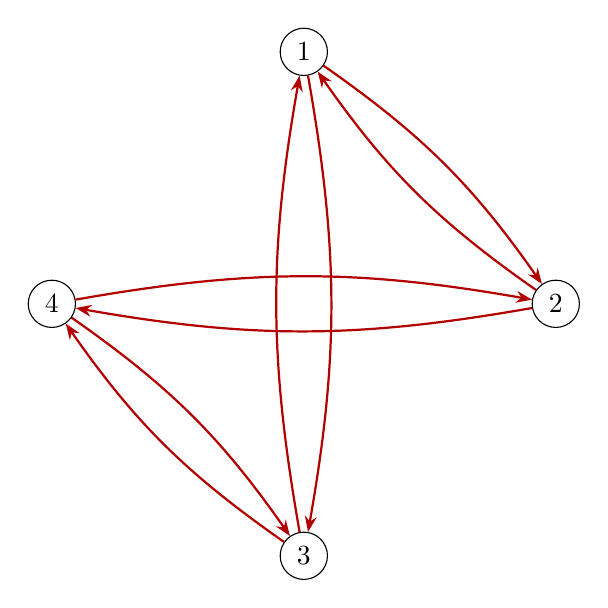
\begin{tikzpicture}[>={Stealth[length=2mm]}]
\node[draw,circle,minimum size=6mm,inner sep=0pt] (n0) at (0.00,3.20) {1};
\node[draw,circle,minimum size=6mm,inner sep=0pt] (n1) at (3.20,0.00) {2};
\node[draw,circle,minimum size=6mm,inner sep=0pt] (n2) at (0.00,-3.20) {3};
\node[draw,circle,minimum size=6mm,inner sep=0pt] (n3) at (-3.20,0.00) {4};
\draw[->,red!70!black,thick] (n0) to[bend left=10] (n1);
\draw[->,red!70!black,thick] (n0) to[bend left=10] (n2);
\draw[->,red!70!black,thick] (n1) to[bend left=10] (n0);
\draw[->,red!70!black,thick] (n1) to[bend left=10] (n3);
\draw[->,red!70!black,thick] (n2) to[bend left=10] (n0);
\draw[->,red!70!black,thick] (n2) to[bend left=10] (n3);
\draw[->,red!70!black,thick] (n3) to[bend left=10] (n1);
\draw[->,red!70!black,thick] (n3) to[bend left=10] (n2);
\end{tikzpicture}
\end{center}
\noindent Solid: defeats. Dashed: supports. Dotted: one party's case is part of another's.
\begin{enumerate}
\item At conversion (Dunn, Stott)
\item After conversion (Assemblies of God; Menzies, Stronstad)
\item A second work of grace (the holiness tradition)
\item In baptism and confirmation (Catholic)
\end{enumerate}
\begin{longtable}{@{}>{\raggedright\arraybackslash}p{0.3\textwidth} >{\raggedright\arraybackslash}p{0.3\textwidth} >{\raggedright\arraybackslash}p{0.3\textwidth}@{}}
\toprule
\textbf{From} & \textbf{To} & \textbf{Edge} \\
\midrule
\endhead
1 \emph{At conversion (Dunn, Stott)} & 2 \emph{After conversion (Assemblies of God; Menzies, Stronstad)} & defeats \\
1 \emph{At conversion (Dunn, Stott)} & 3 \emph{A second work of grace (the holiness tradition)} & defeats \\
2 \emph{After conversion (Assemblies of God; Menzies, Stronstad)} & 1 \emph{At conversion (Dunn, Stott)} & defeats \\
2 \emph{After conversion (Assemblies of God; Menzies, Stronstad)} & 4 \emph{In baptism and confirmation (Catholic)} & defeats \\
3 \emph{A second work of grace (the holiness tradition)} & 1 \emph{At conversion (Dunn, Stott)} & defeats \\
3 \emph{A second work of grace (the holiness tradition)} & 4 \emph{In baptism and confirmation (Catholic)} & defeats \\
4 \emph{In baptism and confirmation (Catholic)} & 2 \emph{After conversion (Assemblies of God; Menzies, Stronstad)} & defeats \\
4 \emph{In baptism and confirmation (Catholic)} & 3 \emph{A second work of grace (the holiness tradition)} & defeats \\
\bottomrule
\end{longtable}
\noindent The defeats are the cells of \texttt{spirit\allowbreak{}Baptism\allowbreak{}Dispute\_\allowbreak{}defeats}, the supports the cells of \texttt{spirit\allowbreak{}Baptism\allowbreak{}Dispute\_\allowbreak{}supports} and the parts the cells of \texttt{spirit\allowbreak{}Baptism\allowbreak{}Dispute\_\allowbreak{}part\allowbreak{}Of}, each computed from the parties' premises and checked by the kernel. The attacks derived through support and through parts are reported, not counted: every verdict is computed from the defeats alone. Every derived attack is already a defeat.
\par\medskip\noindent\textbf{\texttt{conversion\_\allowbreak{}stands\_\allowbreak{}with\_\allowbreak{}the\_\allowbreak{}sacraments}}\par\nobreak\noindent
\textbf{The conversion and sacramental views can be held together}: one reading satisfies both — every believer baptized in the Spirit at conversion, the Spirit given in the sacraments, and no second baptism to seek.

It does not show that the two agree. They differ over what the rite does, which this dispute does not weigh, and the result says only that nothing encoded here makes them contradict each other.

{\small\begin{verbatim}
theorem conversion_stands_with_the_sacraments :
    spiritBaptismDispute.StandTogether [View.conversion, View.sacramental]
-- axioms: propext, Classical.choice, Quot.sound
\end{verbatim}}
\par\medskip\noindent\textbf{\texttt{the\_\allowbreak{}subsequence\_\allowbreak{}views\_\allowbreak{}stand\_\allowbreak{}together}}\par\nobreak\noindent
\textbf{The two subsequence views can be held together}: a second baptism to seek, whether read as empowerment or as the second work of grace. Whether it is the same second experience, the encoding does not say.

{\small\begin{verbatim}
theorem the_subsequence_views_stand_together :
    spiritBaptismDispute.StandTogether [View.pentecostal, View.holiness]
-- axioms: propext, Classical.choice, Quot.sound
\end{verbatim}}
\paragraph*{What the dispute decides}
\leavevmode\par\nobreak
\par\medskip\noindent\textbf{\texttt{spirit\allowbreak{}Baptism\allowbreak{}Settles\allowbreak{}Nothing}}\par\nobreak\noindent
Why nothing is forced: every view has a defeater. The conversion view has the Pentecostal, the Pentecostal and holiness views have the conversion view, and the sacramental view has the Pentecostal.

\paragraph{Nothing prevails outright: every party is defeated by another.}
\begin{itemize}
\item \emph{After conversion (Assemblies of God; Menzies, Stronstad)} defeats \emph{At conversion (Dunn, Stott)}.
\item \emph{At conversion (Dunn, Stott)} defeats \emph{After conversion (Assemblies of God; Menzies, Stronstad)}.
\item \emph{At conversion (Dunn, Stott)} defeats \emph{A second work of grace (the holiness tradition)}.
\item \emph{After conversion (Assemblies of God; Menzies, Stronstad)} defeats \emph{In baptism and confirmation (Catholic)}.
\end{itemize}
\par\noindent\textbf{What this rests on.} The reasons state 4 defeats and 0 absences of defeat, each a cell of the defeat table, \texttt{spirit\allowbreak{}Baptism\allowbreak{}Dispute\_\allowbreak{}defeats}, computed from the two parties' premises and checked by the kernel. Whether an attack survives turns on the attacker's weakest link and on the rating of what it attacks, so a changed rating can change the verdict. The weakest links:
\begin{itemize}
\item \emph{After conversion (Assemblies of God; Menzies, Stronstad)}, weakest at \emph{disputed}:
\begin{itemize}
\item 1 Corinthians 12:13 is baptism by the Spirit into the body, not Christ baptizing in the Spirit --- \cite{assemblies-of-god-baptism-holy-spirit-2010}
\item Acts 8:14–17 and 19:1–7 — believers, already baptized, receive the Spirit afterwards (so the Assemblies of God; Dunn denies they were yet believers) --- \cite{assemblies-of-god-baptism-holy-spirit-2010}; Acts 8:14-17; Acts 19:1-7
\item In Luke-Acts, baptism in the Spirit is prophetic empowerment, distinct from the gift Paul ties to conversion --- \cite{menzies-lukes-understanding-2017}; \cite{menzies-empowered-witness-1994}; \cite{stronstad-charismatic-theology-1984}
\item Luke’s narratives of receiving the Spirit are a pattern for believers today --- \cite{stronstad-charismatic-theology-1984}; \cite{assemblies-of-god-baptism-holy-spirit-2010}
\item an inference step --- \cite{assemblies-of-god-baptism-holy-spirit-2010}; \cite{dunn-baptism-holy-spirit-1970}; \cite{stott-baptism-fullness-1975}
\end{itemize}
\item \emph{At conversion (Dunn, Stott)}, weakest at \emph{disputed}:
\begin{itemize}
\item 1 Corinthians 12:13 is the baptism in the Spirit Christ gives, received by every believer at conversion --- \cite{dunn-baptism-holy-spirit-1970}; \cite{stott-baptism-fullness-1975}
\item an inference step --- \cite{dunn-baptism-holy-spirit-1970}; \cite{stott-baptism-fullness-1975}; \cite{assemblies-of-god-baptism-holy-spirit-2010}
\item an inference step --- \cite{menzies-lukes-understanding-2017}; \cite{menzies-empowered-witness-1994}
\end{itemize}
\item \emph{A second work of grace (the holiness tradition)}, weakest at \emph{disputed}:
\begin{itemize}
\item Entire sanctification is a second work of grace after justification --- \cite[Articles of Faith, X, ¶10]{church-of-the-nazarene-manual-2023}; \cite[to Joseph Benson, 28 December 1770]{wesley-letters-1931}; \cite{bassett-white-paper-article-x-2010}
\item an inference step --- \cite[to Joseph Benson, 28 December 1770]{wesley-letters-1931}; \cite{bassett-white-paper-article-x-2010}
\end{itemize}
\item \emph{In baptism and confirmation (Catholic)}, weakest at \emph{disputed}:
\begin{itemize}
\item The Spirit is given in water baptism: new birth in the Holy Spirit --- \cite[1262]{catholic-church-catechism-2000}; \cite[1265]{catholic-church-catechism-2000}; \cite[Small Catechism, Baptism, third part]{kolb-wengert-book-of-concord-2000}
\item Confirmation gives the full outpouring of the Spirit, as at Pentecost and in Samaria --- \cite[1302]{catholic-church-catechism-2000}; \cite[1288]{catholic-church-catechism-2000}
\item an inference step --- \cite[1302]{catholic-church-catechism-2000}; \cite[XXVIII.6]{westminster-confession-1647}
\item an inference step --- \cite[1302]{catholic-church-catechism-2000}
\end{itemize}
\end{itemize}
\par\medskip\noindent\textbf{\texttt{spirit\_\allowbreak{}baptism\_\allowbreak{}forces\_\allowbreak{}nothing}}\par\nobreak\noindent
\textbf{Nothing is forced.} Every view is in a standoff the dispute cannot resolve, and every weakest link is \texttt{disputed}, so no rating breaks a tie.

It does not show that the question is idle. Each view can be defended, and what the dispute cannot do is choose between readings rated alike.

{\small\begin{verbatim}
theorem spirit_baptism_forces_nothing : Framework.grounded
    spiritBaptismDispute.defeats = ∅
-- axioms: propext, Classical.choice, Quot.sound
\end{verbatim}}
\par\medskip\noindent\textbf{\texttt{conversion\allowbreak{}Stands\allowbreak{}With\allowbreak{}The\allowbreak{}Sacraments}}\par\nobreak\noindent
Why the conversion view can be defended: it stands with the sacramental view, and answers both subsequence views, itself.

\paragraph{\emph{At conversion (Dunn, Stott)} is accepted on some resolution.}
\begin{itemize}
\item A position holding \emph{At conversion (Dunn, Stott)}, \emph{In baptism and confirmation (Catholic)} can be held.
\item None of \emph{At conversion (Dunn, Stott)}, \emph{In baptism and confirmation (Catholic)} defeats another, and each attack on them is answered from among them:
\begin{itemize}
\item \emph{After conversion (Assemblies of God; Menzies, Stronstad)} defeats \emph{At conversion (Dunn, Stott)}, and \emph{At conversion (Dunn, Stott)} defeats \emph{After conversion (Assemblies of God; Menzies, Stronstad)}.
\item \emph{A second work of grace (the holiness tradition)} defeats \emph{At conversion (Dunn, Stott)}, and \emph{At conversion (Dunn, Stott)} defeats \emph{A second work of grace (the holiness tradition)}.
\item \emph{After conversion (Assemblies of God; Menzies, Stronstad)} defeats \emph{In baptism and confirmation (Catholic)}, and \emph{At conversion (Dunn, Stott)} defeats \emph{After conversion (Assemblies of God; Menzies, Stronstad)}.
\item \emph{A second work of grace (the holiness tradition)} defeats \emph{In baptism and confirmation (Catholic)}, and \emph{At conversion (Dunn, Stott)} defeats \emph{A second work of grace (the holiness tradition)}.
\end{itemize}
\end{itemize}
\par\noindent\textbf{What this rests on.} The reasons state 6 defeats and 4 absences of defeat, each a cell of the defeat table, \texttt{spirit\allowbreak{}Baptism\allowbreak{}Dispute\_\allowbreak{}defeats}, computed from the two parties' premises and checked by the kernel. Whether an attack survives turns on the attacker's weakest link and on the rating of what it attacks, so a changed rating can change the verdict. The weakest links:
\begin{itemize}
\item \emph{At conversion (Dunn, Stott)}, weakest at \emph{disputed}:
\begin{itemize}
\item 1 Corinthians 12:13 is the baptism in the Spirit Christ gives, received by every believer at conversion --- \cite{dunn-baptism-holy-spirit-1970}; \cite{stott-baptism-fullness-1975}
\item an inference step --- \cite{dunn-baptism-holy-spirit-1970}; \cite{stott-baptism-fullness-1975}; \cite{assemblies-of-god-baptism-holy-spirit-2010}
\item an inference step --- \cite{menzies-lukes-understanding-2017}; \cite{menzies-empowered-witness-1994}
\end{itemize}
\item \emph{In baptism and confirmation (Catholic)}, weakest at \emph{disputed}:
\begin{itemize}
\item The Spirit is given in water baptism: new birth in the Holy Spirit --- \cite[1262]{catholic-church-catechism-2000}; \cite[1265]{catholic-church-catechism-2000}; \cite[Small Catechism, Baptism, third part]{kolb-wengert-book-of-concord-2000}
\item Confirmation gives the full outpouring of the Spirit, as at Pentecost and in Samaria --- \cite[1302]{catholic-church-catechism-2000}; \cite[1288]{catholic-church-catechism-2000}
\item an inference step --- \cite[1302]{catholic-church-catechism-2000}; \cite[XXVIII.6]{westminster-confession-1647}
\item an inference step --- \cite[1302]{catholic-church-catechism-2000}
\end{itemize}
\item \emph{After conversion (Assemblies of God; Menzies, Stronstad)}, weakest at \emph{disputed}:
\begin{itemize}
\item 1 Corinthians 12:13 is baptism by the Spirit into the body, not Christ baptizing in the Spirit --- \cite{assemblies-of-god-baptism-holy-spirit-2010}
\item Acts 8:14–17 and 19:1–7 — believers, already baptized, receive the Spirit afterwards (so the Assemblies of God; Dunn denies they were yet believers) --- \cite{assemblies-of-god-baptism-holy-spirit-2010}; Acts 8:14-17; Acts 19:1-7
\item In Luke-Acts, baptism in the Spirit is prophetic empowerment, distinct from the gift Paul ties to conversion --- \cite{menzies-lukes-understanding-2017}; \cite{menzies-empowered-witness-1994}; \cite{stronstad-charismatic-theology-1984}
\item Luke’s narratives of receiving the Spirit are a pattern for believers today --- \cite{stronstad-charismatic-theology-1984}; \cite{assemblies-of-god-baptism-holy-spirit-2010}
\item an inference step --- \cite{assemblies-of-god-baptism-holy-spirit-2010}; \cite{dunn-baptism-holy-spirit-1970}; \cite{stott-baptism-fullness-1975}
\end{itemize}
\item \emph{A second work of grace (the holiness tradition)}, weakest at \emph{disputed}:
\begin{itemize}
\item Entire sanctification is a second work of grace after justification --- \cite[Articles of Faith, X, ¶10]{church-of-the-nazarene-manual-2023}; \cite[to Joseph Benson, 28 December 1770]{wesley-letters-1931}; \cite{bassett-white-paper-article-x-2010}
\item an inference step --- \cite[to Joseph Benson, 28 December 1770]{wesley-letters-1931}; \cite{bassett-white-paper-article-x-2010}
\end{itemize}
\end{itemize}
\par\medskip\noindent\textbf{\texttt{conversion\_\allowbreak{}defensible}}\par\nobreak\noindent
\textbf{The conversion view can be defended}, with the sacramental view: some maximal defensible position — one no other party can join without losing that — holds both.

{\small\begin{verbatim}
theorem conversion_defensible : Framework.CredulouslyAccepted
    spiritBaptismDispute.defeats View.conversion
-- axioms: propext, Classical.choice, Quot.sound
\end{verbatim}}
\par\medskip\noindent\textbf{\texttt{conversion\allowbreak{}Answered\allowbreak{}By\allowbreak{}Pentecost}}\par\nobreak\noindent
Why the conversion view is not forced: a defensible position holds the Pentecostal view, and it defeats the conversion view.

\paragraph{\emph{At conversion (Dunn, Stott)} is not accepted on every resolution.}
\begin{itemize}
\item A position holding \emph{After conversion (Assemblies of God; Menzies, Stronstad)}, \emph{A second work of grace (the holiness tradition)} can be held, and it holds \emph{After conversion (Assemblies of God; Menzies, Stronstad)}; \emph{After conversion (Assemblies of God; Menzies, Stronstad)} conflicts with \emph{At conversion (Dunn, Stott)}: \emph{After conversion (Assemblies of God; Menzies, Stronstad)} defeats \emph{At conversion (Dunn, Stott)}, and \emph{At conversion (Dunn, Stott)} defeats \emph{After conversion (Assemblies of God; Menzies, Stronstad)}.
\item None of \emph{After conversion (Assemblies of God; Menzies, Stronstad)}, \emph{A second work of grace (the holiness tradition)} defeats another, and each attack on them is answered from among them:
\begin{itemize}
\item \emph{At conversion (Dunn, Stott)} defeats \emph{After conversion (Assemblies of God; Menzies, Stronstad)}, and \emph{After conversion (Assemblies of God; Menzies, Stronstad)} defeats \emph{At conversion (Dunn, Stott)}.
\item \emph{In baptism and confirmation (Catholic)} defeats \emph{After conversion (Assemblies of God; Menzies, Stronstad)}, and \emph{After conversion (Assemblies of God; Menzies, Stronstad)} defeats \emph{In baptism and confirmation (Catholic)}.
\item \emph{At conversion (Dunn, Stott)} defeats \emph{A second work of grace (the holiness tradition)}, and \emph{After conversion (Assemblies of God; Menzies, Stronstad)} defeats \emph{At conversion (Dunn, Stott)}.
\item \emph{In baptism and confirmation (Catholic)} defeats \emph{A second work of grace (the holiness tradition)}, and \emph{After conversion (Assemblies of God; Menzies, Stronstad)} defeats \emph{In baptism and confirmation (Catholic)}.
\end{itemize}
\end{itemize}
\par\noindent\textbf{What this rests on.} The reasons state 6 defeats and 4 absences of defeat, each a cell of the defeat table, \texttt{spirit\allowbreak{}Baptism\allowbreak{}Dispute\_\allowbreak{}defeats}, computed from the two parties' premises and checked by the kernel. Whether an attack survives turns on the attacker's weakest link and on the rating of what it attacks, so a changed rating can change the verdict. The weakest links:
\begin{itemize}
\item \emph{After conversion (Assemblies of God; Menzies, Stronstad)}, weakest at \emph{disputed}:
\begin{itemize}
\item 1 Corinthians 12:13 is baptism by the Spirit into the body, not Christ baptizing in the Spirit --- \cite{assemblies-of-god-baptism-holy-spirit-2010}
\item Acts 8:14–17 and 19:1–7 — believers, already baptized, receive the Spirit afterwards (so the Assemblies of God; Dunn denies they were yet believers) --- \cite{assemblies-of-god-baptism-holy-spirit-2010}; Acts 8:14-17; Acts 19:1-7
\item In Luke-Acts, baptism in the Spirit is prophetic empowerment, distinct from the gift Paul ties to conversion --- \cite{menzies-lukes-understanding-2017}; \cite{menzies-empowered-witness-1994}; \cite{stronstad-charismatic-theology-1984}
\item Luke’s narratives of receiving the Spirit are a pattern for believers today --- \cite{stronstad-charismatic-theology-1984}; \cite{assemblies-of-god-baptism-holy-spirit-2010}
\item an inference step --- \cite{assemblies-of-god-baptism-holy-spirit-2010}; \cite{dunn-baptism-holy-spirit-1970}; \cite{stott-baptism-fullness-1975}
\end{itemize}
\item \emph{At conversion (Dunn, Stott)}, weakest at \emph{disputed}:
\begin{itemize}
\item 1 Corinthians 12:13 is the baptism in the Spirit Christ gives, received by every believer at conversion --- \cite{dunn-baptism-holy-spirit-1970}; \cite{stott-baptism-fullness-1975}
\item an inference step --- \cite{dunn-baptism-holy-spirit-1970}; \cite{stott-baptism-fullness-1975}; \cite{assemblies-of-god-baptism-holy-spirit-2010}
\item an inference step --- \cite{menzies-lukes-understanding-2017}; \cite{menzies-empowered-witness-1994}
\end{itemize}
\item \emph{A second work of grace (the holiness tradition)}, weakest at \emph{disputed}:
\begin{itemize}
\item Entire sanctification is a second work of grace after justification --- \cite[Articles of Faith, X, ¶10]{church-of-the-nazarene-manual-2023}; \cite[to Joseph Benson, 28 December 1770]{wesley-letters-1931}; \cite{bassett-white-paper-article-x-2010}
\item an inference step --- \cite[to Joseph Benson, 28 December 1770]{wesley-letters-1931}; \cite{bassett-white-paper-article-x-2010}
\end{itemize}
\item \emph{In baptism and confirmation (Catholic)}, weakest at \emph{disputed}:
\begin{itemize}
\item The Spirit is given in water baptism: new birth in the Holy Spirit --- \cite[1262]{catholic-church-catechism-2000}; \cite[1265]{catholic-church-catechism-2000}; \cite[Small Catechism, Baptism, third part]{kolb-wengert-book-of-concord-2000}
\item Confirmation gives the full outpouring of the Spirit, as at Pentecost and in Samaria --- \cite[1302]{catholic-church-catechism-2000}; \cite[1288]{catholic-church-catechism-2000}
\item an inference step --- \cite[1302]{catholic-church-catechism-2000}; \cite[XXVIII.6]{westminster-confession-1647}
\item an inference step --- \cite[1302]{catholic-church-catechism-2000}
\end{itemize}
\end{itemize}
\par\medskip\noindent\textbf{\texttt{conversion\_\allowbreak{}not\_\allowbreak{}forced}}\par\nobreak\noindent
\textbf{Nor is it forced.} A maximal defensible position holds the Pentecostal and holiness views, and cannot hold the conversion view with them.

{\small\begin{verbatim}
theorem conversion_not_forced : ¬Framework.SkepticallyAccepted
    spiritBaptismDispute.defeats View.conversion
-- axioms: propext, Classical.choice, Quot.sound
\end{verbatim}}
\par\medskip\noindent\textbf{\texttt{pentecostal\allowbreak{}Stands\allowbreak{}With\allowbreak{}Holiness}}\par\nobreak\noindent
Why the Pentecostal view can be defended: it stands with the holiness view, and answers both the conversion and sacramental views itself.

\paragraph{\emph{After conversion (Assemblies of God; Menzies, Stronstad)} is accepted on some resolution.}
\begin{itemize}
\item A position holding \emph{After conversion (Assemblies of God; Menzies, Stronstad)}, \emph{A second work of grace (the holiness tradition)} can be held.
\item None of \emph{After conversion (Assemblies of God; Menzies, Stronstad)}, \emph{A second work of grace (the holiness tradition)} defeats another, and each attack on them is answered from among them:
\begin{itemize}
\item \emph{At conversion (Dunn, Stott)} defeats \emph{After conversion (Assemblies of God; Menzies, Stronstad)}, and \emph{After conversion (Assemblies of God; Menzies, Stronstad)} defeats \emph{At conversion (Dunn, Stott)}.
\item \emph{In baptism and confirmation (Catholic)} defeats \emph{After conversion (Assemblies of God; Menzies, Stronstad)}, and \emph{After conversion (Assemblies of God; Menzies, Stronstad)} defeats \emph{In baptism and confirmation (Catholic)}.
\item \emph{At conversion (Dunn, Stott)} defeats \emph{A second work of grace (the holiness tradition)}, and \emph{After conversion (Assemblies of God; Menzies, Stronstad)} defeats \emph{At conversion (Dunn, Stott)}.
\item \emph{In baptism and confirmation (Catholic)} defeats \emph{A second work of grace (the holiness tradition)}, and \emph{After conversion (Assemblies of God; Menzies, Stronstad)} defeats \emph{In baptism and confirmation (Catholic)}.
\end{itemize}
\end{itemize}
\par\noindent\textbf{What this rests on.} The reasons state 6 defeats and 4 absences of defeat, each a cell of the defeat table, \texttt{spirit\allowbreak{}Baptism\allowbreak{}Dispute\_\allowbreak{}defeats}, computed from the two parties' premises and checked by the kernel. Whether an attack survives turns on the attacker's weakest link and on the rating of what it attacks, so a changed rating can change the verdict. The weakest links:
\begin{itemize}
\item \emph{After conversion (Assemblies of God; Menzies, Stronstad)}, weakest at \emph{disputed}:
\begin{itemize}
\item 1 Corinthians 12:13 is baptism by the Spirit into the body, not Christ baptizing in the Spirit --- \cite{assemblies-of-god-baptism-holy-spirit-2010}
\item Acts 8:14–17 and 19:1–7 — believers, already baptized, receive the Spirit afterwards (so the Assemblies of God; Dunn denies they were yet believers) --- \cite{assemblies-of-god-baptism-holy-spirit-2010}; Acts 8:14-17; Acts 19:1-7
\item In Luke-Acts, baptism in the Spirit is prophetic empowerment, distinct from the gift Paul ties to conversion --- \cite{menzies-lukes-understanding-2017}; \cite{menzies-empowered-witness-1994}; \cite{stronstad-charismatic-theology-1984}
\item Luke’s narratives of receiving the Spirit are a pattern for believers today --- \cite{stronstad-charismatic-theology-1984}; \cite{assemblies-of-god-baptism-holy-spirit-2010}
\item an inference step --- \cite{assemblies-of-god-baptism-holy-spirit-2010}; \cite{dunn-baptism-holy-spirit-1970}; \cite{stott-baptism-fullness-1975}
\end{itemize}
\item \emph{A second work of grace (the holiness tradition)}, weakest at \emph{disputed}:
\begin{itemize}
\item Entire sanctification is a second work of grace after justification --- \cite[Articles of Faith, X, ¶10]{church-of-the-nazarene-manual-2023}; \cite[to Joseph Benson, 28 December 1770]{wesley-letters-1931}; \cite{bassett-white-paper-article-x-2010}
\item an inference step --- \cite[to Joseph Benson, 28 December 1770]{wesley-letters-1931}; \cite{bassett-white-paper-article-x-2010}
\end{itemize}
\item \emph{At conversion (Dunn, Stott)}, weakest at \emph{disputed}:
\begin{itemize}
\item 1 Corinthians 12:13 is the baptism in the Spirit Christ gives, received by every believer at conversion --- \cite{dunn-baptism-holy-spirit-1970}; \cite{stott-baptism-fullness-1975}
\item an inference step --- \cite{dunn-baptism-holy-spirit-1970}; \cite{stott-baptism-fullness-1975}; \cite{assemblies-of-god-baptism-holy-spirit-2010}
\item an inference step --- \cite{menzies-lukes-understanding-2017}; \cite{menzies-empowered-witness-1994}
\end{itemize}
\item \emph{In baptism and confirmation (Catholic)}, weakest at \emph{disputed}:
\begin{itemize}
\item The Spirit is given in water baptism: new birth in the Holy Spirit --- \cite[1262]{catholic-church-catechism-2000}; \cite[1265]{catholic-church-catechism-2000}; \cite[Small Catechism, Baptism, third part]{kolb-wengert-book-of-concord-2000}
\item Confirmation gives the full outpouring of the Spirit, as at Pentecost and in Samaria --- \cite[1302]{catholic-church-catechism-2000}; \cite[1288]{catholic-church-catechism-2000}
\item an inference step --- \cite[1302]{catholic-church-catechism-2000}; \cite[XXVIII.6]{westminster-confession-1647}
\item an inference step --- \cite[1302]{catholic-church-catechism-2000}
\end{itemize}
\end{itemize}
\par\medskip\noindent\textbf{\texttt{pentecostal\_\allowbreak{}defensible}}\par\nobreak\noindent
\textbf{The Pentecostal view can be defended}, with the holiness view.

{\small\begin{verbatim}
theorem pentecostal_defensible : Framework.CredulouslyAccepted
    spiritBaptismDispute.defeats View.pentecostal
-- axioms: propext, Classical.choice, Quot.sound
\end{verbatim}}
\par\medskip\noindent\textbf{\texttt{pentecostal\allowbreak{}Answered\allowbreak{}By\allowbreak{}Conversion}}\par\nobreak\noindent
Why the Pentecostal view is not forced: a defensible position holds the conversion view, and it defeats the Pentecostal view.

\paragraph{\emph{After conversion (Assemblies of God; Menzies, Stronstad)} is not accepted on every resolution.}
\begin{itemize}
\item A position holding \emph{At conversion (Dunn, Stott)}, \emph{In baptism and confirmation (Catholic)} can be held, and it holds \emph{At conversion (Dunn, Stott)}; \emph{At conversion (Dunn, Stott)} conflicts with \emph{After conversion (Assemblies of God; Menzies, Stronstad)}: \emph{At conversion (Dunn, Stott)} defeats \emph{After conversion (Assemblies of God; Menzies, Stronstad)}, and \emph{After conversion (Assemblies of God; Menzies, Stronstad)} defeats \emph{At conversion (Dunn, Stott)}.
\item None of \emph{At conversion (Dunn, Stott)}, \emph{In baptism and confirmation (Catholic)} defeats another, and each attack on them is answered from among them:
\begin{itemize}
\item \emph{After conversion (Assemblies of God; Menzies, Stronstad)} defeats \emph{At conversion (Dunn, Stott)}, and \emph{At conversion (Dunn, Stott)} defeats \emph{After conversion (Assemblies of God; Menzies, Stronstad)}.
\item \emph{A second work of grace (the holiness tradition)} defeats \emph{At conversion (Dunn, Stott)}, and \emph{At conversion (Dunn, Stott)} defeats \emph{A second work of grace (the holiness tradition)}.
\item \emph{After conversion (Assemblies of God; Menzies, Stronstad)} defeats \emph{In baptism and confirmation (Catholic)}, and \emph{At conversion (Dunn, Stott)} defeats \emph{After conversion (Assemblies of God; Menzies, Stronstad)}.
\item \emph{A second work of grace (the holiness tradition)} defeats \emph{In baptism and confirmation (Catholic)}, and \emph{At conversion (Dunn, Stott)} defeats \emph{A second work of grace (the holiness tradition)}.
\end{itemize}
\end{itemize}
\par\noindent\textbf{What this rests on.} The reasons state 6 defeats and 4 absences of defeat, each a cell of the defeat table, \texttt{spirit\allowbreak{}Baptism\allowbreak{}Dispute\_\allowbreak{}defeats}, computed from the two parties' premises and checked by the kernel. Whether an attack survives turns on the attacker's weakest link and on the rating of what it attacks, so a changed rating can change the verdict. The weakest links:
\begin{itemize}
\item \emph{At conversion (Dunn, Stott)}, weakest at \emph{disputed}:
\begin{itemize}
\item 1 Corinthians 12:13 is the baptism in the Spirit Christ gives, received by every believer at conversion --- \cite{dunn-baptism-holy-spirit-1970}; \cite{stott-baptism-fullness-1975}
\item an inference step --- \cite{dunn-baptism-holy-spirit-1970}; \cite{stott-baptism-fullness-1975}; \cite{assemblies-of-god-baptism-holy-spirit-2010}
\item an inference step --- \cite{menzies-lukes-understanding-2017}; \cite{menzies-empowered-witness-1994}
\end{itemize}
\item \emph{After conversion (Assemblies of God; Menzies, Stronstad)}, weakest at \emph{disputed}:
\begin{itemize}
\item 1 Corinthians 12:13 is baptism by the Spirit into the body, not Christ baptizing in the Spirit --- \cite{assemblies-of-god-baptism-holy-spirit-2010}
\item Acts 8:14–17 and 19:1–7 — believers, already baptized, receive the Spirit afterwards (so the Assemblies of God; Dunn denies they were yet believers) --- \cite{assemblies-of-god-baptism-holy-spirit-2010}; Acts 8:14-17; Acts 19:1-7
\item In Luke-Acts, baptism in the Spirit is prophetic empowerment, distinct from the gift Paul ties to conversion --- \cite{menzies-lukes-understanding-2017}; \cite{menzies-empowered-witness-1994}; \cite{stronstad-charismatic-theology-1984}
\item Luke’s narratives of receiving the Spirit are a pattern for believers today --- \cite{stronstad-charismatic-theology-1984}; \cite{assemblies-of-god-baptism-holy-spirit-2010}
\item an inference step --- \cite{assemblies-of-god-baptism-holy-spirit-2010}; \cite{dunn-baptism-holy-spirit-1970}; \cite{stott-baptism-fullness-1975}
\end{itemize}
\item \emph{In baptism and confirmation (Catholic)}, weakest at \emph{disputed}:
\begin{itemize}
\item The Spirit is given in water baptism: new birth in the Holy Spirit --- \cite[1262]{catholic-church-catechism-2000}; \cite[1265]{catholic-church-catechism-2000}; \cite[Small Catechism, Baptism, third part]{kolb-wengert-book-of-concord-2000}
\item Confirmation gives the full outpouring of the Spirit, as at Pentecost and in Samaria --- \cite[1302]{catholic-church-catechism-2000}; \cite[1288]{catholic-church-catechism-2000}
\item an inference step --- \cite[1302]{catholic-church-catechism-2000}; \cite[XXVIII.6]{westminster-confession-1647}
\item an inference step --- \cite[1302]{catholic-church-catechism-2000}
\end{itemize}
\item \emph{A second work of grace (the holiness tradition)}, weakest at \emph{disputed}:
\begin{itemize}
\item Entire sanctification is a second work of grace after justification --- \cite[Articles of Faith, X, ¶10]{church-of-the-nazarene-manual-2023}; \cite[to Joseph Benson, 28 December 1770]{wesley-letters-1931}; \cite{bassett-white-paper-article-x-2010}
\item an inference step --- \cite[to Joseph Benson, 28 December 1770]{wesley-letters-1931}; \cite{bassett-white-paper-article-x-2010}
\end{itemize}
\end{itemize}
\par\medskip\noindent\textbf{\texttt{pentecostal\_\allowbreak{}not\_\allowbreak{}forced}}\par\nobreak\noindent
\textbf{Nor is it forced.} A maximal defensible position holds the conversion and sacramental views, and cannot hold the Pentecostal view with them. What would decide is argued, not weighed: what the Acts narratives are (\texttt{pentecostal\_\allowbreak{}cannot\_\allowbreak{}read\_\allowbreak{}acts\_\allowbreak{}as\_\allowbreak{}transitions}).

{\small\begin{verbatim}
theorem pentecostal_not_forced : ¬Framework.SkepticallyAccepted
    spiritBaptismDispute.defeats View.pentecostal
-- axioms: propext, Classical.choice, Quot.sound
\end{verbatim}}
\par\medskip\noindent\textbf{\texttt{holiness\allowbreak{}Stands\allowbreak{}With\allowbreak{}Pentecost}}\par\nobreak\noindent
Why the holiness view can be defended: it stands with the Pentecostal view, which answers the conversion and sacramental views.

\paragraph{\emph{A second work of grace (the holiness tradition)} is accepted on some resolution.}
\begin{itemize}
\item A position holding \emph{After conversion (Assemblies of God; Menzies, Stronstad)}, \emph{A second work of grace (the holiness tradition)} can be held.
\item None of \emph{After conversion (Assemblies of God; Menzies, Stronstad)}, \emph{A second work of grace (the holiness tradition)} defeats another, and each attack on them is answered from among them:
\begin{itemize}
\item \emph{At conversion (Dunn, Stott)} defeats \emph{After conversion (Assemblies of God; Menzies, Stronstad)}, and \emph{After conversion (Assemblies of God; Menzies, Stronstad)} defeats \emph{At conversion (Dunn, Stott)}.
\item \emph{In baptism and confirmation (Catholic)} defeats \emph{After conversion (Assemblies of God; Menzies, Stronstad)}, and \emph{After conversion (Assemblies of God; Menzies, Stronstad)} defeats \emph{In baptism and confirmation (Catholic)}.
\item \emph{At conversion (Dunn, Stott)} defeats \emph{A second work of grace (the holiness tradition)}, and \emph{After conversion (Assemblies of God; Menzies, Stronstad)} defeats \emph{At conversion (Dunn, Stott)}.
\item \emph{In baptism and confirmation (Catholic)} defeats \emph{A second work of grace (the holiness tradition)}, and \emph{After conversion (Assemblies of God; Menzies, Stronstad)} defeats \emph{In baptism and confirmation (Catholic)}.
\end{itemize}
\end{itemize}
\par\noindent\textbf{What this rests on.} The reasons state 6 defeats and 4 absences of defeat, each a cell of the defeat table, \texttt{spirit\allowbreak{}Baptism\allowbreak{}Dispute\_\allowbreak{}defeats}, computed from the two parties' premises and checked by the kernel. Whether an attack survives turns on the attacker's weakest link and on the rating of what it attacks, so a changed rating can change the verdict. The weakest links:
\begin{itemize}
\item \emph{After conversion (Assemblies of God; Menzies, Stronstad)}, weakest at \emph{disputed}:
\begin{itemize}
\item 1 Corinthians 12:13 is baptism by the Spirit into the body, not Christ baptizing in the Spirit --- \cite{assemblies-of-god-baptism-holy-spirit-2010}
\item Acts 8:14–17 and 19:1–7 — believers, already baptized, receive the Spirit afterwards (so the Assemblies of God; Dunn denies they were yet believers) --- \cite{assemblies-of-god-baptism-holy-spirit-2010}; Acts 8:14-17; Acts 19:1-7
\item In Luke-Acts, baptism in the Spirit is prophetic empowerment, distinct from the gift Paul ties to conversion --- \cite{menzies-lukes-understanding-2017}; \cite{menzies-empowered-witness-1994}; \cite{stronstad-charismatic-theology-1984}
\item Luke’s narratives of receiving the Spirit are a pattern for believers today --- \cite{stronstad-charismatic-theology-1984}; \cite{assemblies-of-god-baptism-holy-spirit-2010}
\item an inference step --- \cite{assemblies-of-god-baptism-holy-spirit-2010}; \cite{dunn-baptism-holy-spirit-1970}; \cite{stott-baptism-fullness-1975}
\end{itemize}
\item \emph{A second work of grace (the holiness tradition)}, weakest at \emph{disputed}:
\begin{itemize}
\item Entire sanctification is a second work of grace after justification --- \cite[Articles of Faith, X, ¶10]{church-of-the-nazarene-manual-2023}; \cite[to Joseph Benson, 28 December 1770]{wesley-letters-1931}; \cite{bassett-white-paper-article-x-2010}
\item an inference step --- \cite[to Joseph Benson, 28 December 1770]{wesley-letters-1931}; \cite{bassett-white-paper-article-x-2010}
\end{itemize}
\item \emph{At conversion (Dunn, Stott)}, weakest at \emph{disputed}:
\begin{itemize}
\item 1 Corinthians 12:13 is the baptism in the Spirit Christ gives, received by every believer at conversion --- \cite{dunn-baptism-holy-spirit-1970}; \cite{stott-baptism-fullness-1975}
\item an inference step --- \cite{dunn-baptism-holy-spirit-1970}; \cite{stott-baptism-fullness-1975}; \cite{assemblies-of-god-baptism-holy-spirit-2010}
\item an inference step --- \cite{menzies-lukes-understanding-2017}; \cite{menzies-empowered-witness-1994}
\end{itemize}
\item \emph{In baptism and confirmation (Catholic)}, weakest at \emph{disputed}:
\begin{itemize}
\item The Spirit is given in water baptism: new birth in the Holy Spirit --- \cite[1262]{catholic-church-catechism-2000}; \cite[1265]{catholic-church-catechism-2000}; \cite[Small Catechism, Baptism, third part]{kolb-wengert-book-of-concord-2000}
\item Confirmation gives the full outpouring of the Spirit, as at Pentecost and in Samaria --- \cite[1302]{catholic-church-catechism-2000}; \cite[1288]{catholic-church-catechism-2000}
\item an inference step --- \cite[1302]{catholic-church-catechism-2000}; \cite[XXVIII.6]{westminster-confession-1647}
\item an inference step --- \cite[1302]{catholic-church-catechism-2000}
\end{itemize}
\end{itemize}
\par\medskip\noindent\textbf{\texttt{holiness\_\allowbreak{}defensible}}\par\nobreak\noindent
\textbf{The holiness view can be defended}, with the Pentecostal view. Not forced, for the same reason the Pentecostal view is not.

{\small\begin{verbatim}
theorem holiness_defensible : Framework.CredulouslyAccepted
    spiritBaptismDispute.defeats View.holiness
-- axioms: propext, Classical.choice, Quot.sound
\end{verbatim}}
\par\medskip\noindent\textbf{\texttt{sacramental\allowbreak{}Stands\allowbreak{}With\allowbreak{}Conversion}}\par\nobreak\noindent
Why the sacramental view can be defended: it stands with the conversion view, which answers both subsequence views.

\paragraph{\emph{In baptism and confirmation (Catholic)} is accepted on some resolution.}
\begin{itemize}
\item A position holding \emph{At conversion (Dunn, Stott)}, \emph{In baptism and confirmation (Catholic)} can be held.
\item None of \emph{At conversion (Dunn, Stott)}, \emph{In baptism and confirmation (Catholic)} defeats another, and each attack on them is answered from among them:
\begin{itemize}
\item \emph{After conversion (Assemblies of God; Menzies, Stronstad)} defeats \emph{At conversion (Dunn, Stott)}, and \emph{At conversion (Dunn, Stott)} defeats \emph{After conversion (Assemblies of God; Menzies, Stronstad)}.
\item \emph{A second work of grace (the holiness tradition)} defeats \emph{At conversion (Dunn, Stott)}, and \emph{At conversion (Dunn, Stott)} defeats \emph{A second work of grace (the holiness tradition)}.
\item \emph{After conversion (Assemblies of God; Menzies, Stronstad)} defeats \emph{In baptism and confirmation (Catholic)}, and \emph{At conversion (Dunn, Stott)} defeats \emph{After conversion (Assemblies of God; Menzies, Stronstad)}.
\item \emph{A second work of grace (the holiness tradition)} defeats \emph{In baptism and confirmation (Catholic)}, and \emph{At conversion (Dunn, Stott)} defeats \emph{A second work of grace (the holiness tradition)}.
\end{itemize}
\end{itemize}
\par\noindent\textbf{What this rests on.} The reasons state 6 defeats and 4 absences of defeat, each a cell of the defeat table, \texttt{spirit\allowbreak{}Baptism\allowbreak{}Dispute\_\allowbreak{}defeats}, computed from the two parties' premises and checked by the kernel. Whether an attack survives turns on the attacker's weakest link and on the rating of what it attacks, so a changed rating can change the verdict. The weakest links:
\begin{itemize}
\item \emph{At conversion (Dunn, Stott)}, weakest at \emph{disputed}:
\begin{itemize}
\item 1 Corinthians 12:13 is the baptism in the Spirit Christ gives, received by every believer at conversion --- \cite{dunn-baptism-holy-spirit-1970}; \cite{stott-baptism-fullness-1975}
\item an inference step --- \cite{dunn-baptism-holy-spirit-1970}; \cite{stott-baptism-fullness-1975}; \cite{assemblies-of-god-baptism-holy-spirit-2010}
\item an inference step --- \cite{menzies-lukes-understanding-2017}; \cite{menzies-empowered-witness-1994}
\end{itemize}
\item \emph{In baptism and confirmation (Catholic)}, weakest at \emph{disputed}:
\begin{itemize}
\item The Spirit is given in water baptism: new birth in the Holy Spirit --- \cite[1262]{catholic-church-catechism-2000}; \cite[1265]{catholic-church-catechism-2000}; \cite[Small Catechism, Baptism, third part]{kolb-wengert-book-of-concord-2000}
\item Confirmation gives the full outpouring of the Spirit, as at Pentecost and in Samaria --- \cite[1302]{catholic-church-catechism-2000}; \cite[1288]{catholic-church-catechism-2000}
\item an inference step --- \cite[1302]{catholic-church-catechism-2000}; \cite[XXVIII.6]{westminster-confession-1647}
\item an inference step --- \cite[1302]{catholic-church-catechism-2000}
\end{itemize}
\item \emph{After conversion (Assemblies of God; Menzies, Stronstad)}, weakest at \emph{disputed}:
\begin{itemize}
\item 1 Corinthians 12:13 is baptism by the Spirit into the body, not Christ baptizing in the Spirit --- \cite{assemblies-of-god-baptism-holy-spirit-2010}
\item Acts 8:14–17 and 19:1–7 — believers, already baptized, receive the Spirit afterwards (so the Assemblies of God; Dunn denies they were yet believers) --- \cite{assemblies-of-god-baptism-holy-spirit-2010}; Acts 8:14-17; Acts 19:1-7
\item In Luke-Acts, baptism in the Spirit is prophetic empowerment, distinct from the gift Paul ties to conversion --- \cite{menzies-lukes-understanding-2017}; \cite{menzies-empowered-witness-1994}; \cite{stronstad-charismatic-theology-1984}
\item Luke’s narratives of receiving the Spirit are a pattern for believers today --- \cite{stronstad-charismatic-theology-1984}; \cite{assemblies-of-god-baptism-holy-spirit-2010}
\item an inference step --- \cite{assemblies-of-god-baptism-holy-spirit-2010}; \cite{dunn-baptism-holy-spirit-1970}; \cite{stott-baptism-fullness-1975}
\end{itemize}
\item \emph{A second work of grace (the holiness tradition)}, weakest at \emph{disputed}:
\begin{itemize}
\item Entire sanctification is a second work of grace after justification --- \cite[Articles of Faith, X, ¶10]{church-of-the-nazarene-manual-2023}; \cite[to Joseph Benson, 28 December 1770]{wesley-letters-1931}; \cite{bassett-white-paper-article-x-2010}
\item an inference step --- \cite[to Joseph Benson, 28 December 1770]{wesley-letters-1931}; \cite{bassett-white-paper-article-x-2010}
\end{itemize}
\end{itemize}
\par\medskip\noindent\textbf{\texttt{sacramental\_\allowbreak{}defensible}}\par\nobreak\noindent
\textbf{The sacramental view can be defended}, with the conversion view. Not forced, for the same reason the conversion view is not.

{\small\begin{verbatim}
theorem sacramental_defensible : Framework.CredulouslyAccepted
    spiritBaptismDispute.defeats View.sacramental
-- axioms: propext, Classical.choice, Quot.sound
\end{verbatim}}
\paragraph*{What the Pentecostal view can read Acts as}
\leavevmode\par\nobreak
\par\medskip\noindent\textbf{\texttt{pentecostal\_\allowbreak{}cannot\_\allowbreak{}read\_\allowbreak{}acts\_\allowbreak{}as\_\allowbreak{}transitions}}\par\nobreak\noindent
\textbf{The Pentecostal view cannot read Acts as transitions.} Its own premise is that Luke’s narratives are a pattern for believers today, and Stott’s reading says, in its own words, that they are “not a pattern” (\texttt{Testimony\allowbreak{}Arguments.Meanings.Spirit\allowbreak{}Baptism.joins}). So what the view holds, read for what its claims mean, denies the transitions reading outright.

So the Pentecostal view must read the Acts narratives as a pattern, because the other reading is not open to it. It does not show that the pattern reading is right. Read as a pattern, the narratives still meet the variety of Acts (\texttt{where\allowbreak{}The\allowbreak{}Variety\allowbreak{}Meets\allowbreak{}The\allowbreak{}Pattern}), at a step the Assemblies of God contest.

Before the two readings were joined by meaning, this was a dilemma with two horns, and the transitions horn broke only at Stott’s step from transitions to no norm. Joined, the horn is not there to break: no reader can hold the Pentecostal view and read Acts as transitions.

{\small\begin{verbatim}
theorem pentecostal_cannot_read_acts_as_transitions : Entails
    pentecostalCase.held (notP Claim.actsEpisodesAreTransitions)
-- axioms: propext, Quot.sound
\end{verbatim}}
\par\medskip\noindent\textbf{\texttt{stott\_\allowbreak{}undermines\_\allowbreak{}the\_\allowbreak{}pattern}}\par\nobreak\noindent
\textbf{Stott’s reading meets the Pentecostal view at its premise.} Read for what its claims mean, Acts as transitions denies that the narratives are a pattern, and that is one of the Pentecostal view’s premises. Before the join it met the view only at Stott’s step, as a reason not to seek a second baptism; now it contradicts what the view rests on. Whether that attack is a defeat is a question of ratings, and this argument’s dispute does not seat Stott’s reading as a party.

{\small\begin{verbatim}
theorem stott_undermines_the_pattern : UnderminesOn transitionCase
    pentecostalCase (p Claim.actsNarrativesAreNormative)
-- axioms: propext, Quot.sound
\end{verbatim}}
\subsection*{Appendix: the claims and their sources}
\addcontentsline{toc}{subsection}{Appendix: the claims and their sources}
The texts each side reads, the readings each side gives them, and the three conclusions the four views reach (the two subsequence views share one). The texts are kept apart from the readings, so that a reader can see which claims are what Luke and Paul say and which are what a tradition says they mean.

\subsubsection*{Citation and classification for every atom}
Every claim must name a source, or the encoding will not build (\texttt{cite}). Each reading is cited to a source that holds it. Each step’s rating is cited to a reader who accepts the claims it starts from (its grounds) and still denies where it ends, or says that no such reader was found.

\subsubsection*{The claims, numbered}
\begin{longtable}{@{}r >{\raggedright\arraybackslash}p{0.30\textwidth} l >{\raggedright\arraybackslash}p{0.19\textwidth} >{\raggedright\arraybackslash}p{0.21\textwidth}@{}}
\toprule
 & claim & kind & held & source \\
\midrule
\endhead
\pvartarget{TestimonyArguments.SpiritBaptism}{1}$P_{1}$ & 1 Corinthians 12:13 — in one Spirit we were all baptized into one body\textsuperscript{\dag} & textual & Christian, hist.-gramm., consensus & 1 Cor 12:13 \\
\pvartarget{TestimonyArguments.SpiritBaptism}{2}$P_{2}$ & Acts 8:14–17 and 19:1–7 — believers, already baptized, receive the Spirit afterwards (so the Assemblies of God; Dunn denies they were yet believers) & textual & Christian, hist.-gramm., disputed & \cite{assemblies-of-god-baptism-holy-spirit-2010}; Acts 8:14-17; Acts 19:1-7 \\
\pvartarget{TestimonyArguments.SpiritBaptism}{3}$P_{3}$ & Acts 10:44–48 — the Spirit falls on Cornelius’s household before baptism\textsuperscript{\dag} & textual & Christian, hist.-gramm., consensus & Acts 10:44-48 \\
\pvartarget{TestimonyArguments.SpiritBaptism}{4}$P_{4}$ & Acts 2:38 — repent and be baptized, and you will receive the gift of the Spirit\textsuperscript{\dag} & textual & Christian, hist.-gramm., consensus & Acts 2:38 \\
\pvartarget{TestimonyArguments.SpiritBaptism}{5}$P_{5}$ & 1 Corinthians 12:13 is the baptism in the Spirit Christ gives, received by every believer at conversion & interpretive & Christian, hist.-gramm., disputed & \cite{dunn-baptism-holy-spirit-1970}; \cite{stott-baptism-fullness-1975} \\
\pvartarget{TestimonyArguments.SpiritBaptism}{6}$P_{6}$ & 1 Corinthians 12:13 is baptism by the Spirit into the body, not Christ baptizing in the Spirit & interpretive & Christian, hist.-gramm., disputed & \cite{assemblies-of-god-baptism-holy-spirit-2010} \\
\pvartarget{TestimonyArguments.SpiritBaptism}{7}$P_{7}$ & In Luke-Acts, baptism in the Spirit is prophetic empowerment, distinct from the gift Paul ties to conversion & interpretive & Christian, hist.-gramm., disputed & \cite{menzies-lukes-understanding-2017}; \cite{menzies-empowered-witness-1994}; \cite{stronstad-charismatic-theology-1984} \\
\pvartarget{TestimonyArguments.SpiritBaptism}{8}$P_{8}$ & Luke’s narratives of receiving the Spirit are a pattern for believers today & interpretive & Christian, hist.-gramm., disputed & \cite{stronstad-charismatic-theology-1984}; \cite{assemblies-of-god-baptism-holy-spirit-2010} \\
\pvartarget{TestimonyArguments.SpiritBaptism}{9}$P_{9}$ & The episodes of Acts 8, 10 and 19 are unrepeatable steps in the gospel’s spread, not a pattern & interpretive & Christian, hist.-gramm., disputed & \cite{stott-baptism-fullness-1975} \\
\pvartarget{TestimonyArguments.SpiritBaptism}{10}$P_{10}$ & Entire sanctification is a second work of grace after justification & theological & Christian, hist.-gramm., disputed & \cite[Articles of Faith, X, ¶10]{church-of-the-nazarene-manual-2023}; \cite[to Joseph Benson, 28 December 1770]{wesley-letters-1931}; \cite{bassett-white-paper-article-x-2010} \\
\pvartarget{TestimonyArguments.SpiritBaptism}{11}$P_{11}$ & The Spirit is given in water baptism: new birth in the Holy Spirit & theological & Roman Catholic, disputed & \cite[1262]{catholic-church-catechism-2000}; \cite[1265]{catholic-church-catechism-2000}; \cite[Small Catechism, Baptism, third part]{kolb-wengert-book-of-concord-2000} \\
\pvartarget{TestimonyArguments.SpiritBaptism}{12}$P_{12}$ & Confirmation gives the full outpouring of the Spirit, as at Pentecost and in Samaria & theological & Roman Catholic, disputed & \cite[1302]{catholic-church-catechism-2000}; \cite[1288]{catholic-church-catechism-2000} \\
\pvartarget{TestimonyArguments.SpiritBaptism}{13}$P_{13}$ & Every believer is baptized in the Spirit at conversion & theological & Christian, hist.-gramm., disputed & \cite{dunn-baptism-holy-spirit-1970}; \cite{stott-baptism-fullness-1975} \\
\pvartarget{TestimonyArguments.SpiritBaptism}{14}$P_{14}$ & A baptism in the Spirit distinct from and after conversion is to be sought & theological & Christian, hist.-gramm., disputed & \cite{assemblies-of-god-baptism-holy-spirit-2010}; \cite[Articles of Faith, X, ¶10]{church-of-the-nazarene-manual-2023} \\
\pvartarget{TestimonyArguments.SpiritBaptism}{15}$P_{15}$ & The Spirit is given in baptism and confirmation, not in a second baptism beyond the sacraments & theological & Roman Catholic, disputed & \cite[1302]{catholic-church-catechism-2000} \\
\bottomrule
\end{longtable}

\noindent\footnotesize \textsuperscript{\dag} grounded in scripture alone: the reading is assumed, not argued for.
\normalsize
\subsubsection*{How this is checked}
\paragraph*{Ratings for inference steps}
\leavevmode\par\nobreak
\par\medskip\noindent\textbf{\texttt{on\allowbreak{}The\allowbreak{}Conversion\allowbreak{}Step}}\par\nobreak\noindent
\textbf{The step from 1 Corinthians 12:13 to Spirit baptism at conversion is rated \texttt{disputed}, conservatively.} Dunn and Stott hold it. The Assemblies of God reject its conclusion, but by denying a ground — that the verse speaks of Christ baptizing in the Spirit: “‘by’ is the best translation, indicating that the Holy Spirit is the instrument” — so they do not contest the step itself. No reader was sought who grants both grounds and denies the conclusion, so the step is not rated above the bottom.

{\small\begin{verbatim}
def onTheConversionStep : Source :=
  { primary := Reference.work dunnBaptismInTheHolySpirit,
    supporting :=
      [Reference.work stottBaptismAndFullness,
        Reference.work agBaptismPositionPaper],
    tradition := Tradition.christianHistoricalGrammatical,
    confidence := Confidence.disputed }
\end{verbatim}}
\par\medskip\noindent\textbf{\texttt{menzies\allowbreak{}Against\allowbreak{}No\allowbreak{}Second}}\par\nobreak\noindent
\textbf{The step from Spirit baptism at conversion to “no second to seek” is contested, by Menzies.} He grants that Paul’s baptism in the Spirit at 1 Corinthians 12:13 is tied to conversion, and holds that Luke’s is a different, prophetic gift, to be sought after it. Whether that is granting the ground and denying the conclusion, or reading “baptism in the Spirit” in two senses, is the question of Paul’s word and Luke’s, which this argument does not yet encode.

{\small\begin{verbatim}
def menziesAgainstNoSecond : Source :=
  { primary := Reference.work menziesLukesUnderstanding,
    supporting := [Reference.work menziesEmpoweredForWitness],
    tradition := Tradition.christianHistoricalGrammatical,
    confidence := Confidence.disputed }
\end{verbatim}}
\par\medskip\noindent\textbf{\texttt{on\allowbreak{}The\allowbreak{}Instrumental\allowbreak{}Step}}\par\nobreak\noindent
\textbf{The step from the Pentecostal reading of 1 Corinthians 12:13 is rated \texttt{disputed}, conservatively.} The Assemblies of God hold it. Dunn and Stott reject its conclusion, but by denying a ground — they read the verse as the baptism in the Spirit that Christ gives, not the Spirit as instrument — so they do not contest the step itself. No reader was sought who grants both grounds and denies the conclusion, so the step is not rated above the bottom.

{\small\begin{verbatim}
def onTheInstrumentalStep : Source :=
  { primary := Reference.work agBaptismPositionPaper,
    supporting :=
      [Reference.work dunnBaptismInTheHolySpirit,
        Reference.work stottBaptismAndFullness],
    tradition := Tradition.christianHistoricalGrammatical,
    confidence := Confidence.disputed }
\end{verbatim}}
\par\medskip\noindent\textbf{\texttt{acts\allowbreak{}To\allowbreak{}Subsequence}}\par\nobreak\noindent
\textbf{The step from the Acts narratives to a second Spirit baptism is well supported}: grant that believers in Samaria and Ephesus received the Spirit later, that Luke’s Spirit baptism is empowerment, and that his narratives are a pattern, and the conclusion follows. Unlike the steps rated conservatively here, this one was audited for a reader who grants all three grounds and denies the conclusion, and none was found: the readers who reject it deny a ground — Dunn, that the Samaritans were yet Christians; Stott and Fee, that the narratives are a pattern. The other steps were not audited in their encoded form, so they stay at the bottom.

{\small\begin{verbatim}
def actsToSubsequence : Source :=
  { primary := Reference.work agBaptismPositionPaper,
    supporting := [Reference.work stronstadCharismaticTheology],
    tradition := Tradition.christianHistoricalGrammatical,
    confidence := Confidence.wellSupported }
\end{verbatim}}
\par\medskip\noindent\textbf{\texttt{wesley\allowbreak{}Against\allowbreak{}The\allowbreak{}Holiness\allowbreak{}Name}}\par\nobreak\noindent
\textbf{The holiness step is contested, from within the Wesleyan tradition.} The Church of the Nazarene holds it (\emph{Manual} 2023, Article X). Wesley grants the “second change, whereby they shall be saved from all sin and perfected in love”, and denies that it is Spirit baptism: “If they like to call this ‘receiving the Holy Ghost,’ they may: only the phrase in that sense is not scriptural and not quite proper; for they all ‘received the Holy Ghost’ when they were justified” (to Joseph Benson, 28 December 1770). The Nazarene seminary faculty, keeping entire sanctification, “no longer view the American holiness hermeneutic of the ‘baptism of the Spirit’ as exegetically tenable” (2010).

{\small\begin{verbatim}
def wesleyAgainstTheHolinessName : Source :=
  {
    primary :=
      Reference.work wesleyLetters
        (Bib.Locus.sectionRef "to Joseph Benson, 28 December 1770"),
    supporting := [Reference.work nazareneWhitePaper],
    tradition := Tradition.christianHistoricalGrammatical,
    confidence := Confidence.disputed }
\end{verbatim}}
\par\medskip\noindent\textbf{\texttt{on\allowbreak{}The\allowbreak{}Rite}}\par\nobreak\noindent
\textbf{The sacramental step is rated \texttt{disputed}, conservatively.} Rome holds it (Catechism 1302). Westminster rejects the sacramental view, but by denying a ground — that the Spirit is given in the rite as Rome says: baptism’s efficacy “is not tied to that moment of time wherein it is administered” (XXVIII.6) — so it does not contest the step itself. No reader was sought who grants the grounds and denies the conclusion, so the step is not rated above the bottom.

{\small\begin{verbatim}
def onTheRite : Source :=
  {
    primary :=
      Reference.work catechismCatholicChurch (Bib.Locus.sectionRef "1302"),
    supporting :=
      [Reference.work westminsterConfession (Bib.Locus.sectionRef "XXVIII.6")],
    tradition := Tradition.romanCatholic, confidence := Confidence.disputed }
\end{verbatim}}
\par\medskip\noindent\textbf{\texttt{on\allowbreak{}The\allowbreak{}Sacramental\allowbreak{}Exclusion}}\par\nobreak\noindent
\textbf{The step from the Spirit given in the sacraments to “no second baptism to seek” is rated \texttt{disputed}, conservatively.} Rome holds it (Catechism 1302). The natural contester is the Catholic charismatic renewal, which keeps the sacramental gift and speaks of a “baptism in the Spirit” of its own; its texts were not verified, so it is not cited, and the step is not rated above the bottom.

{\small\begin{verbatim}
def onTheSacramentalExclusion : Source :=
  {
    primary :=
      Reference.work catechismCatholicChurch (Bib.Locus.sectionRef "1302"),
    tradition := Tradition.romanCatholic, confidence := Confidence.disputed }
\end{verbatim}}
\par\medskip\noindent\textbf{\texttt{ag\allowbreak{}Against\allowbreak{}The\allowbreak{}Variety}}\par\nobreak\noindent
\textbf{The step from the variety of Acts is contested, by the Assemblies of God.} They grant Acts 10 and 2:38 and still read Acts as a pattern: their paper lists Acts 10:44–46 among the evidence \emph{for} a subsequent experience.

{\small\begin{verbatim}
def agAgainstTheVariety : Source :=
  { primary := Reference.work agBaptismPositionPaper,
    tradition := Tradition.christianHistoricalGrammatical,
    confidence := Confidence.disputed }
\end{verbatim}}
\par\medskip\noindent\textbf{\texttt{stott\allowbreak{}On\allowbreak{}The\allowbreak{}Transitions}}\par\nobreak\noindent
\textbf{The step from the transitions reading is rated \texttt{disputed}, conservatively.} If the episodes of Acts are unrepeatable, they set no norm for believers today, Stott argues. No reader was sought who grants the transitions reading and still holds a second Spirit baptism to be the norm, so the step is not rated above the bottom.

{\small\begin{verbatim}
def stottOnTheTransitions : Source :=
  { primary := Reference.work stottBaptismAndFullness,
    tradition := Tradition.christianHistoricalGrammatical,
    confidence := Confidence.disputed }
\end{verbatim}}
\paragraph*{Citations}
\leavevmode\par\nobreak
\par\medskip\noindent\textbf{\texttt{cite}}\par\nobreak\noindent
Citation and classification for every atom. Total, so nothing is uncited.

{\small\begin{verbatim}
def cite : Claim → AtomMeta
\end{verbatim}}

\bibliographystyle{plain}
\bibliography{references}
\end{document}
